% Tratto da grfguide.[ps|pdf]:
%
%\graphicspath{<dir-list>}
%    This optional declaration may be used to specify a list of directories in which to search
%    for graphics files. The format is the same as for the LATEX 2e primitive \input@path.
%    A list of directories, each in a {} group (even if there is only one in the list). For example:
%    \graphicspath{{eps/}{tiff/}}
%    would cause the system to look in the subdirectories eps and tiff of the current directory.
%
%\graphicspath{{FIGS/}}
%
% E` preferibile fare come segue, perche' in questo modo ad es. anche i .tex
% possono essere messi in altre directory e inclusi senza indicarne il percorso.
\makeatletter
\let\input@path=\@undefined
\def\input@path{{FIGS/}}
\makeatother

\ifx\pdfoutput\undefined % We are not running pdftex
\documentclass[12pt,a4paper]{book}

\usepackage[dvips]{graphicx,color}
% \usepackage{psfig}
% \usepackage{epsfig}
\DeclareGraphicsExtensions{.ps,.eps,.pstex}
% Use the following line if you want to obtain a .pdf through dvipdfm
% (.tex -(latex)-> .dvi -(dvipdfm)-> .pdf)
\RequirePackage[dvipdfm,hyperindex]{hyperref}
% % \RequirePackage[dvipdfm,colorlinks,hyperindex]{hyperref}
% Use the following two lines if you want to obtain a .pdf with hyperlinks
% also through ps2pdf (.tex -(latex)-> .dvi -(dvips)-> .ps -(ps2pdf)-> .pdf)
% (this can be useful if you want to use Inkscape and PSFrag to put
%  equations in the figure)
% \RequirePackage[hyperindex]{hyperref}
% \usepackage{psfrag}
% % \RequirePackage[hypertex]{hyperref}
\else % We are running pdftex
\documentclass[pdftex,12pt,a4paper]{report}
\usepackage[pdftex]{graphicx,color}
\DeclareGraphicsExtensions{.pdf,.png,.jpg,.mps}
\RequirePackage[hyperindex]{hyperref}
% % \RequirePackage[colorlinks,hyperindex]{hyperref}
% % \usepackage{thumbpdf}
\hypersetup{
pdftitle={Progetto e caratterizzazione di un dispositivo elettromagnetico per il rilevamento
della disponibilità di parcheggio},
pdfsubject={Tesi Laurea Triennale},
pdfauthor={Giacomo Mammarella},
pdfkeywords={Modello, tesi, LaTeX, PDF, Howto, pdflatex, dvipdfm},
% pdfpagemode=FullScreen
}
\fi

\usepackage{times}
%\usepackage{mathptmx}
\usepackage[scaled=.90]{helvet}
\usepackage{courier}
\usepackage{float}

\textwidth	140 mm
\textheight	210 mm
\headheight	 10 mm
\headsep	  8 mm
\hoffset	 14.6 mm
\oddsidemargin	  0 mm
\voffset	  9.6 mm
\topmargin	  0 mm
\renewcommand{\baselinestretch}{1.14}
% \renewcommand{\baselinestretch}{1}
% \baselineskip = 20 pt

\date{~}
\newlength{\defaultparindent}
\setlength{\defaultparindent}{\parindent}

\usepackage{enumerate}
\usepackage{float}

\usepackage[italian]{babel}
\usepackage[utf8]{inputenc}
%\usepackage[latin1]{inputenc}
%\usepackage[applemac]{inputenc}

\frenchspacing

\usepackage{amssymb,amstext,amsmath}
%\usepackage{bigint}
%\usepackage{esint}
%\usepackage{multirow}
\usepackage{listings}
\usepackage{color}
\usepackage{subfig}

\newcommand{\ty}{\tilde{y}}
\newcommand{\tM}{\widetilde{M}}
\newcommand{\tSIR}{\text{SIR}}
\newcommand{\tout}{\text{out}}
\newcommand{\thit}{\text{hit}}
\newcommand{\thop}{\text{hop}}
\newcommand{\setawn}{\left( \sigma_{w_n} , \eta_{w_n} \right)}
\newcommand{\var}{\text{var}}
%\def\myvector#1{\underline{#1}}
%\def\myversor#1{\hat{\underline{#1}}}
\newcommand{\myvector}[1]{\underline{#1}}
\newcommand{\myversor}[1]{\hat{\underline{#1}}}
%\newcommand{\myvector}[1]{\text{\boldmath $#1$}}
%\newcommand{\myversor}[1]{\hat{\text{\boldmath $#1$}}}
%\newcommand{\mymatrix}[1]{\text{\boldmath $#1$}}
\newcommand{\mymatrix}[1]{\pmb{#1}}
\newcommand{\erf}{\text{erf}}
\newcommand{\erfc}{\text{erfc}}
\newcommand{\erfinv}{\text{erfinv}}
\newcommand{\inverf}{\text{inverf}}
\newcommand{\rect}{\text{rect}}
\newcommand{\rep}{\text{rep}}
\newcommand{\sinc}{\text{sinc}}
\newcommand{\sgn}{\text{sgn}}
\newcommand{\conv}{\otimes}
\newcommand{\T}{\mathbb{T}}
\newcommand{\R}{\mathbb{R}}
\newcommand{\Z}{\mathbb{Z}}
\newcommand{\C}{\mathbb{C}}
\newcommand{\F}{\mathcal{F}}

\RequirePackage{fancyhdr}
\pagestyle{fancy}
\fancyhf{}
%\renewcommand{\chaptermark}[1]{\markboth{\scshape \chaptername\ \thechapter\ -- #1}{}}
\renewcommand{\chaptermark}[1]{\markboth{\chaptername\ \thechapter\ -- #1}{}}
\fancyhead[L]{\leftmark}
\fancyhead[R]{\thepage}

% Per far numerare anche le subsubsection:
\setcounter{secnumdepth}{3} % il default è 2 e quindi comprende fino alle subsection
% Per far inserire anche le subsubsection nella Table Of Contents:
\setcounter{tocdepth}{3}    % il default è 2 e quindi comprende fino alle subsection

\usepackage{verbatim}

%%MY STYLES
%%%%%%%%%%%
%%  XML  %%
%%%%%%%%%%%
\definecolor{gray}{rgb}{0.4,0.4,0.4}
\definecolor{darkblue}{rgb}{0.0,0.0,0.6}
\definecolor{cyan}{rgb}{0.0,0.6,0.6}
\DeclareFixedFont{\ttb}{T1}{txtt}{bx}{n}{12} % for bold
\DeclareFixedFont{\ttm}{T1}{txtt}{m}{n}{12}  % for normal
\definecolor{deepblue}{rgb}{0,0,0.5}
\definecolor{deepred}{rgb}{0.6,0,0}
\definecolor{deepyellow}{rgb}{0.6,0.6,0}
\definecolor{deepgreen}{rgb}{0,0.5,0}

\lstset{
  basicstyle=\ttfamily,
  columns=fullflexible,
  showstringspaces=false,
  commentstyle=\color{gray}\upshape,
  breaklines=true,
}

\lstdefinelanguage{XML}
{
  morestring=[b]",
  morestring=[s]{>}{<},
  morecomment=[s]{<?}{?>},
  stringstyle=\color{black},
  identifierstyle=\color{darkblue},
  keywordstyle=\color{cyan},
  morekeywords={xmlns,version,type}% list your attributes here
}

%%%%%%%%%%%
%%  PHP  %%
%%%%%%%%%%%
\lstdefinelanguage{PHP}
{
  morestring=[b]",
  morestring=[s]{"}{"},
  stringstyle     =\color{deepgreen},
  identifierstyle =\color{black},
  otherkeywords   = {fopen, fclose, bcadd, fwrite, bccomp, bcsub, true, false, ksort, isset, fgets, round, substr, preg_match, feof, trim, explode},   
  keywordstyle    =\color{darkblue},
  commentstyle    = \color{gray},
  emph            =[1]{php, <?php, ?>},
  emphstyle       =[1]\color{black},
  emph            =[2]{if,and,or,else,while,for, foreach, as},
  emphstyle       =[2]\color{deepred}
}

%%%%%%%%%%%%
%%  BASH  %%
%%%%%%%%%%%%
\lstdefinelanguage{BASH}
{
  stringstyle=\color{black},
  identifierstyle=\color{darkblue},
  commentstyle=\color{red},
  keywordstyle=\color{blue},
  morekeywords={xmlns,version,type}% list your attributes here
}

%%%%%%%%%%%%
%% PYTHON %%
%%%%%%%%%%%%
\lstdefinelanguage{PYTHON}
{
  morestring=[s]{"}{"},
  stringstyle=\color{deepgreen},
  identifierstyle =\color{black},
  basicstyle=\ttm,
  otherkeywords={self, import, def, class, except, open, while, str, handle.write, handle.close},             % Add keywords here
  keywordstyle=\ttb\color{deepblue},
  emph={MyClass,__init__},          % Custom highlighting
  emphstyle=\ttb\color{deepred},    % Custom highlighting style
  frame=tb,                         % Any extra options here
  showstringspaces=false,           % 
}

\graphicspath{{FIGS/}}

\begin{document}

\pagenumbering{arabic}

\setcounter{chapter}{0}
\setcounter{section}{1}

\begin{titlepage}

\begin{center}
\normalsize

\begin{center}
\begin{tabular}[t]{@{} l @{} c @{} r @{}}
\parbox[c]{0.15\textwidth}{\raggedright 
\includegraphics[width=0.75in]{logo_univ}}
&
\parbox[c]{0.7\textwidth}
{
\centering \bfseries
UNIVERSITÀ DEGLI STUDI DELL'AQUILA \\[-5pt]
\rule{0.65\textwidth}{1pt} \\
{\scshape DIPARTIMENTO DI \\ INGEGNERIA INDUSTRIALE E DELL'INFORMAZIONE E DI ECONOMIA }
}
&
\parbox[c]{0.15\textwidth}{\raggedleft 
\includegraphics[width=1.1in]{logo_ing}}
\end{tabular}
\end{center}

\bigskip \bigskip



\bigskip \bigskip

{\small TESINA DI ELETTRONICA DEI SISTEMI DIGITALI 2\\

\vfil \vfil \vfil

{\bfseries \large
Implementazione di metodi di indirizzamento specifici per un sistema digitale a logica programmata\\
}

\vfil \vfil \vfil

Giacomo Mammarella

\vfil \vfil \vfil

\rule{\textwidth}{1pt}\\
{\scshape Anno Accademico 2017--2018}
}
\end{center}

\end{titlepage}


%\input{dedica}
%\input{Sommario}
\newpage

\tableofcontents

\setcounter{page}{1}

\chapter{Introduzione}
\addcontentsline{toc}{chapter}{Introduzione}
La realizzazione di un sistema digitale complesso è possibile mediante due diverse strategie realizzative basilari: la sintesi in \textit{hardware diretto} e la sintesi in \textit{logica programmata}.
Entrambe queste metodologie realizzative, seppur presentando differenze architetturali sostanziali, possono garantire la sintesi di due sistemi digitali assolutamente equivalenti dal punto di vista del legame ingresso-uscita, che mantengano ossia prestazioni funzionali invariate. \newline
La scelta della metodologia di realizzazione di un sistema digitale dipende dalle circostanze strettamente legate alla funzionalità del sistema da realizzare. Ogni soluzione presenta i propri vantaggi e svantaggi ed è compito del progettista verificare che la soluzione adottata sia compatibile con le specifiche imposte dal problema in esame.  \newline

\section*{Logica Programmata}
\addcontentsline{toc}{section}{Logica Programmata}
In generale, un esecutore a logica programmabile è un sistema dotato di un set di istruzioni finito, la cui combinazione appropriata può garantire l'implementazione di algoritmi generici definibili dall'utente.\par \noindent
Il sistema dunque dispone di un'architettura interna in grado di supportare l'esecuzione di istruzioni base, il cui insieme definisce \textit{instruction-set}.
Architettura e set di istruzioni non sono parametri fissi, dunque il ventaglio delle soluzioni disponibili nella realizzazione di un esecutore programmabile è molto ampio, esistendo una molteplicità di soluzioni distinguibili in prima approssimazione secondo i parametri di \textit{area occupata}, \textit{performance} e \textit{potenza dissipata}.\par \noindent
A monte è possibile tuttavia differenziare i sistemi a logica programmabile secondo il tipo di architettura interna adottata. Storicamente, agli albori dello sviluppo dei microcontrollori digitali integrati, nacquero sistemi come l'Intel 4004 basati su un'architettura denominata \textit{archietettura di Von Neumann}, dal nome del matematico che la introdusse. Tale architettura costituisce un esecutore programmabile strettamente sequenziale di tipo master-slave completo ed è internamente strutturata come nella figura seguente.
\begin{figure}[H]
	\centering
	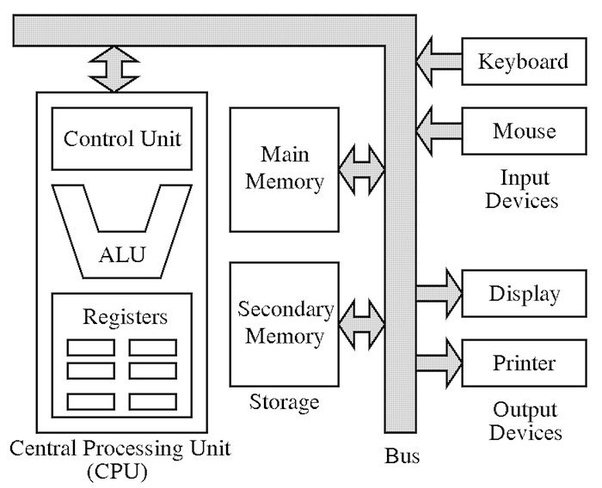
\includegraphics[scale=0.55]{0_von_neumann.png}
	\caption{Architettura di Von Neumann.}
	\label{fig:von_neumann}
\end{figure}

\par %\bigskip
\noindent
La struttura così costituita è composta da tre componenti fondamentali a cui vanno ad aggiungersi le periferiche collegate tramite un modulo di input - output. Tali componenti sono:
\begin{itemize}
	\item Il sistema di memoria, dove risiedono le istruzioni ed i dati necessari all'esecuzione del programma. La memoria può essere costituita da diversi livelli gerarchici. In linea generale si può considerare il \textquotedblleft sistema di memoria" come una memoria principale di tipo RAM nella quale, a runtime, siano già precaricate le istruzioni ed i dati relativi al programma in esecuzione. La memoria può essere vista come un insieme di registri indirizzabili singolarmente e di tipo general purpose, aventi ossia la possibilità di mantenere dati ed istruzioni.
	\item Il sistema di calcolo centralizzato (CPU) che si occupa delle fasi di esecuzione delle istruzioni caricate nella memoria, ossia di eseguire le fasi di FETCH, DECODE, EXECUTE, WRITE BACK per ogni singola istruzione. Al suo interno contiene il sistema di calcolo aritmetico-logico (ALU), l'unità di controllo ed un banco di registri ad alta velocità nel quale i dati vengono salvati mano a mano che viene eseguito il processamento di un'istruzione.
	\item il BUS, che interconnette con la CPU la memoria ed i dispositivi di ingresso - uscita facenti parte del sistema. \'E un bus unico per dati, istruzioni e comandi di controllo, pertanto costituisce un limite prestazionale di tale architettura di calcolo.
\end{itemize}
Come detto su tale architettura è possibile definire un insieme delle istruzioni elementari eseguibili, denominato \textit{instruction-set}. All'interno dell'instruction-set sono disponibili le istruzioni, i registri, le modalità di indirizzamento, l'architettura della memoria, la gestione degli interrupt e delle eccezioni, ed eventualmente l'indirizzamento per i dispositivi di I/O esterni.\\
La combinazione degli elementi presenti all'interno dell'instruction-set in maniera non univoca e più o meno efficiente, permette l'implementazione di un algoritmo fisicamente eseguibile sull'architettura hardware adottata.
L'instruction-set corrisponde dunque a un'interfaccia tra software ed hardware che permette al progettista dell'algoritmo di operare in maniera più semplice sui dispositivi e i segnali interni al sistema digitale col fine dell'implementazione dell'algoritmo stesso.\\
La progettazione dell'instruction-set dipende dall'architettura adottata nel progetto dell'esecutore, differenziando tra sistemi di tipo \textquotedblleft general purpose" come i microprocessori o \textquotedblleft special purpose" come ad esempio i microcontrollori.
A titolo di esempio di un noto set di istruzioni si riporta di seguito quello relativo al microprocessore Intel 4004, il primo microprocessore integrato a 4 bit rilasciato da Intel nel 1971.
\newpage \null \vfill
\begin{figure}[H]
	\centering
	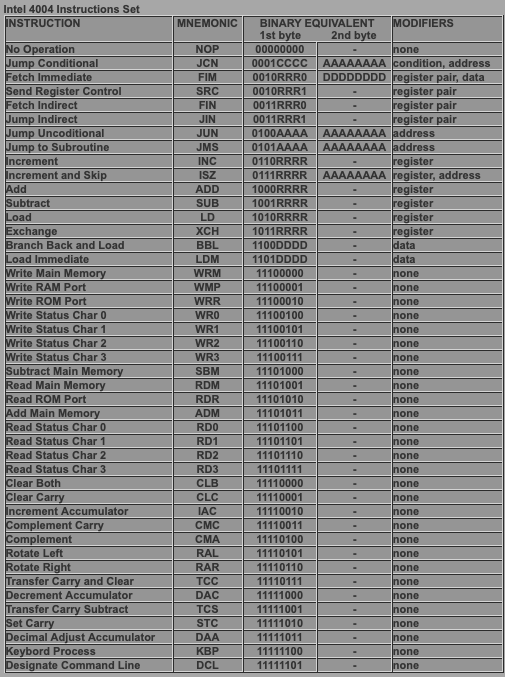
\includegraphics[scale=0.75]{0_4004_instruction_set.png}
	\caption{Il set di istruzioni relativo al microprocessore Intel 4004}
	\label{fig:4004_instruction_set}
\end{figure}
\newpage

\subsection*{Esecuzione delle istruzioni}
\addcontentsline{toc}{subsection}{Esecuzione delle istruzioni}
Sulla base dell'architettura di Von Neumann esposta, a partire dall'instruction-set precedentemente definito, è possibile implementare un algoritmo specifico combinando le istruzioni con i dati che realizzano la funzione desiderata. In prima approssimazione si può pensare che dati e programmi relativi a tale algoritmo siano presenti all'interno della memoria del sistema in maniera sequenziale e sotto forma di linguaggio macchina.\\
Prendendo ad esempio un programma in grado di realizzare la somma tra due valori binari caricati all'interno di altrettanti registri (denominati DR1 e DR2) e il salvataggio del risultato su di un terzo registro (denominato RIS), si avrà il seguente codice assembler:
\begin{lstlisting}[frame=single] 
MV DR1, OP1					 % copia il valore di DR1 in OP1
MV DR2, OP2				 	% salva il valore di DR2 in OP2
SUM				% somma OP1 e OP2 (risultato in ACC)
MV ACC, RIS				% salva il valore di ACC in RIS
\end{lstlisting}
in cui le etichette dei registri corrispondono ad un identificativo hardware (indirizzo) anch'esso definito all'interno dell'instruction-set.
In memoria RAM saranno presenti quindi le istruzioni ed i dati derivanti da tale esempio di programma in maniera sequenziale e come riportato nella figura seguente.
\begin{table}[H]
	\centering
	\begin{tabular}{l|p{2cm}|}
		\cline{2-2} \multicolumn{0}{c|}{0x00} & \makebox[2cm][c]{\textbf{MV}}\\
		\cline{2-2} \multicolumn{0}{c|}{0x01} & \makebox[2cm][c]{DR1}\\
		\cline{2-2} \multicolumn{0}{c|}{0x02} & \makebox[2cm][c]{OP1}\\
		\cline{2-2} \multicolumn{0}{c|}{0x03} & \makebox[2cm][c]{\textbf{MV}}\\
		\cline{2-2} \multicolumn{0}{c|}{0x04} & \makebox[2cm][c]{DR2}\\
		\cline{2-2} \multicolumn{0}{c|}{0x05} & \makebox[2cm][c]{OP2}\\
		\cline{2-2} \multicolumn{0}{c|}{0x06} & \makebox[2cm][c]{\textbf{SUM}}\\
		\cline{2-2} \multicolumn{0}{c|}{0x07} & \makebox[2cm][c]{\textbf{MV}}\\
		\cline{2-2} \multicolumn{0}{c|}{0x07} & \makebox[2cm][c]{ACC}\\
		\cline{2-2} \multicolumn{0}{c|}{0x09} & \makebox[2cm][c]{RIS}\\
		\cline{2-2} \multicolumn{0}{c|}{0x0A} & \makebox[2cm][c]{\textbf{END}}\\
		\cline{2-2} \multicolumn{0}{c|}{} & \makebox[2cm][c]{...}\\
		\multicolumn{0}{c|}{} & \makebox[2cm][c]{...}\\ \cline{2-2}
		\multicolumn{0}{c|}{0xFF} & \makebox[2cm][c]{...}\\ \cline{2-2}
	\end{tabular}
	%\caption*{Organizzazione della memoria relativa al programma d'esempio }
\end{table}
\noindent
L'esecuzione di un'istruzione avviene col ciclo di \textit{fetch-execute}, mantenuto da parte dell'unità di processamento centrale CPU.
Al suo interno sono infatti presenti tutti i sistemi relativi alla sequenziazione delle operazioni (unità di controllo CU), al calcolo aritmetico nonché registri di appoggio dedicati al salvataggio di dati temporanei ed inidirzzamento della memoria.
\begin{figure}[H]
	\centering
	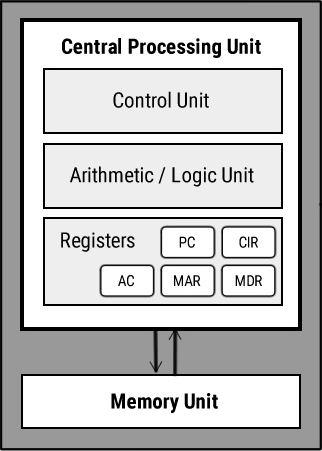
\includegraphics[scale=0.5]{0_vn_cpu.png}
	\caption{La CPU all'interno di un sistema alla Von Neumann}
	\label{fig:vn_cpu}
\end{figure}
\noindent
Nel caso pratico dell'esempio precedentemente riportato, all'avvio dell'esecuzione del programma la CPU darà il comando di \textit{fetch} dell'istruzione presente nella locazione di memoria avente indirizzo 0x00.\\
Al riconoscimento dell'istruzione (\textit{fase di decode}) il sistema diviene al corrente del fatto che ai successivi due prelievi dalla memoria corrisponderanno gli operandi dell'istruzione precedentemente caricata.\\
La fase di \textit{execute} inizia con il prelievo dei dati dagli indirizzi 0x01 e 0x02. Avendo quindi caricato i dati relativi alla prima MOVE il sistema esegue l'istruzione che ha come risultato il salvataggio nel registro denominato OP1 del valore contenuto nel registro denominato DR1.\\
A seguire il sistema esegue a seconda istruzione (prelevata all'indirizzo 0x03 ripetendo quanto detto con la prima MOVE) che termina col salvataggio del dato presente in DR2 sul registro OP2.\\
Al prelievo dell'istruzione all'indirizzo 0x06, corrispondente alla SUM, il sistema esegue la somma dei valori caricati sui registri OP1 ed OP2, precedentemente aggiornati ai valori desiderati. La somma termina col salvataggio del risultato sul registro accumulatore interno (denominato ACC). Infine, con l'istruzione 0x07 si esegue una ulteriore MOVE del dato salvato in ACC sul registro denominato RIS.
Il programma termina con l'esecuzione dell'istruzione all'indirizzo 0x0A e denominata END, che comunica alla macchina il termine delle operazioni del programma.
\par \bigskip
\noindent
L'esecuzione delle istruzioni in questo modello architetturale di memoria prevede il fatto che i dati ed i programmi siano caricati in maniera sequenziale nelle locazioni di memoria. L'indirizzamento della memoria è affidato ad un particolare registro denominato \textquotedblleft Program-Counter", abbreviato con l'identificativo PC. Il valore mantenuto all'interno del PC costituisce quindi l'indirizzo della istruzione in esecuzione o del dato relativo all'istruzione che lo necessita. All'avvenuto prelievo dell'istruzione o del dato corrente (o comunque prima del prelievo della successiva) il PC viene incrementato di 1 puntando di fatto alla successiva locazione di memoria che conterrà un dato o una nuova istruzione.\\
Inoltre poiché si è supposto che l'avvio dell'esecuzione del programma parta dal fetch dell'istruzione all'indirizzo 0x00, allora questa locazione deve necessariamente contenere la prima istruzione che costituisce l'inizio dell'algoritmo.
\par \bigskip \noindent
Quanto detto costituisce un limite prestazionale all'impiego dell'architettura di Von Neumann in quanto la presenza di un unico bus per dati ed istruzioni (e segnali di controllo) limita fortemente le prestazioni di throughput dei dati da parte del sistema. Unitamente a questo limite prestazionale derivante dall'architettura stessa, la gestione della memoria come descritta, ossia contenente i dati relativi alle istruzioni nelle locazioni di memoria strettamente successive alle istruzioni stesse, non permette la realizzazione di tecniche di parallelizzazione volte all'incremento delle prestazioni del sistema.\\ Per tale motivo nel seguente paragrafo verrà descritto un sistema di gestione della memoria più efficiente e compatibile con le tecniche di parallelizzazione.

\subsection*{Von Neumann migliorato}
\addcontentsline{toc}{subsection}{Von Neumann migliorato}
Una soluzione al problema descritto nelle ultime righe del precedente paragrafo prevede la modifica della gestione della memoria nel salvataggio di dati e istruzioni. Questa può essere concettualmente divisa in due aree, una dove vengono salvate in sequenza le istruzioni da eseguire, l'altra che contiene i dati relativi a tali istruzioni, come schematizzato nella figura successiva.
\begin{figure}[H]
	\centering
	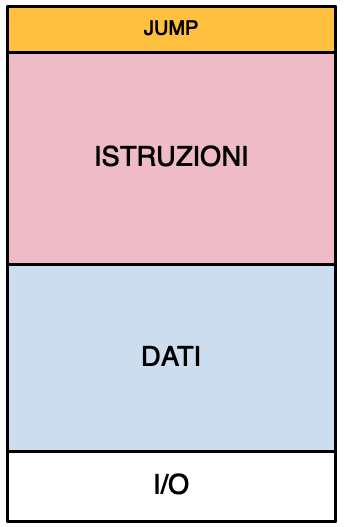
\includegraphics[scale=0.4]{0_memoria_separata.png}
	\caption{Gesione della memoria in un'architettura di Von Neumann migliorata}
	\label{fig:vn_mem}
\end{figure}
\noindent
In tale architettura la gestione della memoria prevede, oltre al classico puntatore all'istruzione denominato program-counter, un puntatore al dato denominato data-counter, abbreviato DC. Tale puntatore contiene l'indirizzo da fornire alla memoria per il prelievo del dato relativo alla istruzione che lo necessita. In questo modo si riescono a garantire due importanti prerogative:
\begin{itemize}
	\item Nel caso in cui non si debba effettuare un salto l'indirizzo relativo alla prossima istruzione è sempre dato dall'indirizzo corrente di PC sommato ad 1.
	\item Nel caso in cui si debba effettuare un salto il valore che punta alla prossima istruzione può già essere puntato da DC e non deve essere ricavato eseguendo un ulteriore aggiornamento di PC per il prelievo di tale dato. In questo modo (nel caso di chiamata a subroutine) il valore di PC può essere salvato come indirizzo di ritorno prima di aggiornare il PC all'indirizzo prelevato dalla memoria e al quale eseguire il salto.
\end{itemize}
L'indirizzamento della memoria si ottiene supponendo delle dimensioni fisse per le aree riservati a istruzioni e dati.\\
Una qualsiasi istruzione presente nell'area dedicata è indirizzabile tramite due coordinate. Una prima fissa, denominata \textit{base istruzione} ed una seconda che indica \textit{l'offset} rispetto a tale base. L'indirizzamento dunque avviene per mezzo del calcolo della seguente somma:
\begin{equation} %\notag
	ADDR_{P} = P_0 + \Delta P
\end{equation} 
Analogamente, in riferimento al calcolo della posizione di un dato si avrà:
\begin{equation}
	ADDR_{D} = D_0 + \Delta D
\end{equation}

\section*{Metodi di indirizzamento}
\label{metodi_di_indirizzamento}
\addcontentsline{toc}{section}{Metodi di indirizzamento}
In base a quanto detto fino ad ora si può procedere alla definizione dell'argomento di questa tesina. Scopo del problema è la progettazione di una UC per un'architettura di Von Neumann curando l'implementazione di parte del set di istruzioni relativo all'indirizzamento della memoria RAM interna, in cui sia prevista la gestione migliorata della memoria precedentemente discussa.\\
In particolare è richiesta l'implementazione delle seguenti istruzioni:
\begin{itemize}
	\item \textbf{RD ADDR}: Esegue una READ della memoria all'indirizzo fornito attraverso il dato ADDR. Il valore letto è salvato su di un registro interno. Per garantire l'indirizzamento di tutto lo spazio di memoria l'operando ADDR è a 2N bit.
	\item \textbf{WR DATA, ADDR}: Esegue la scrittura del valore identificato con DATA nella locuzione di memoria RAM relativa all'indirizzo ADDR. È un'istruzione dal formato \textquotedblleft un'istruzione e due dati".
	Le dimensioni degli operandi: DATA N bit, ADDR 2N bit.
	\item \textbf{JMP ADDR}: Esegue una JUMP incondizionale all'indirizzo presente nel dato ADDR. Tale istruzione realizza un \textquotedblleft \textit{salto immediato}". Il formato dell'istruzione è del tipo \textquotedblleft una istruzione e un dato" ed è a 2N bit.
	\item \textbf{JMP OFFS}: Esegue una JUMP incondizionale all'indirizzo dato dal valore corrente di PC sommato al dato in ingresso denominato OFFS. Costituisce un'istruzione denominata \textquotedblleft \textit{salto diretto}" e prende in ingresso un unico dato. Loperando OFFS ha dimensioni pari a N bit.
	\item \textbf{JMP BASE, OFFS}: Esegue una JUMP incondizionale all'indirizzo calcolato tramite somma dei due dati in ingresso BASE e OFFS. Costituisce un tipo di salto denominato \textquotedblleft \textit{salto indiretto}" e possiede un formato del tipo \textquotedblleft una istruzione e due dati". BASE ed OFFS sono a N bit.
\end{itemize}
Inoltre, dotando la CPU di un insieme di registri interni di tipo \textquotedblleft general-purpose" in appoggio al sistema di calcolo, si implementerà la seguente istruzione:
\begin{itemize}
	\item \textbf{MV REG1, REG2}: Esegue la copia del dato contenuto nel registro avente etichetta REG1 sul registro avente etichetta REG2. Tale istruzione si applica sui registri interni alla CPU.
\end{itemize}

\section*{Istanziazione zero}
\addcontentsline{toc}{section}{Istanziazione zero}
Dunque, in base a quanto esposto precedentemente, si parte con un sistema alla Von Neumann basilare come di seguito nuovamente riportato. All'avvio delle operazioni si suppone che la memoria RAM sia già precaricata con le istruzioni ed i dati nelle aree di memoria dedicate.
\begin{figure}[H]
	\centering
	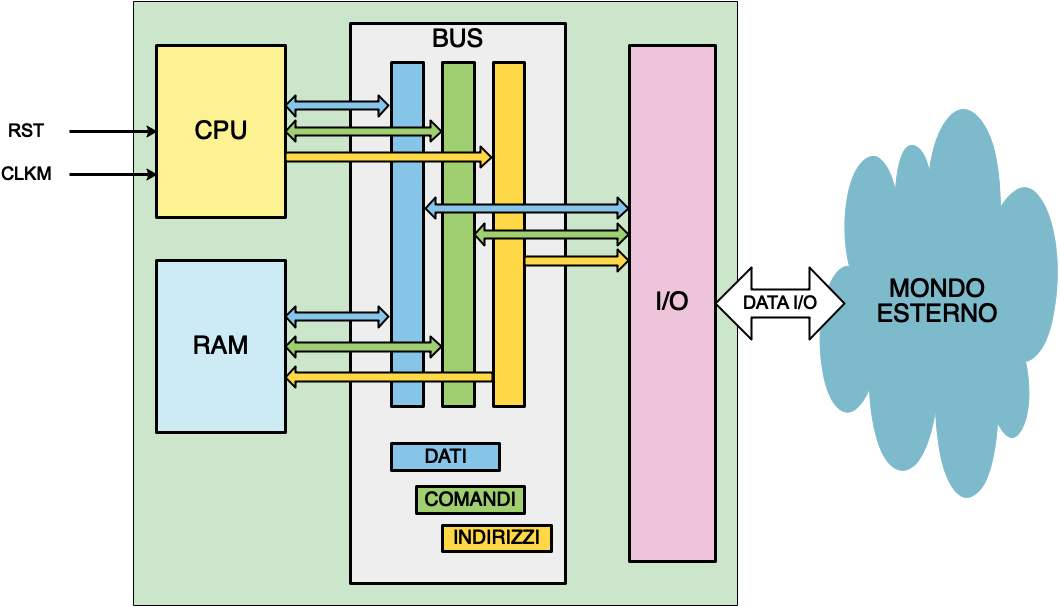
\includegraphics[scale=0.30]{0_ist_zero.png}
	\caption{Struttura interna del sistema in esame}
	\label{fig:ist_0}
\end{figure}
\noindent
Le comunicazioni con l'esterno avvengono per mezzo del bus di I/O ad N bit. Si partirà nello svolgimento del problema tipo \textquotedblleft carta e penna" con un valore per le dimensioni del bus dati pari a $N = 4$. La dimensione del bus indirizzi si sceglie pari a $M=2\cdot N$ bit che definisce uno spazio di indirizzamento della memoria pari a $2^{8} = 256$ parole a N bit. In seguito, su ambiente di sviluppo ISE, si modificherà la dimensione del bus dati (e di conseguenza quella del bus indirizzi) per un valore di N = 8 bit. Dunque i segnali presenti a questo livello di definizione del problema sono i seguenti:
\begin{itemize}
	\item \textbf{OPERANDI E RISULTATO:}
	\begin{itemize}
		\item \textbf{DATA\_IO} (N bit): bus di input-output di collegamento con l'esterno.
	\end{itemize}

	\item \textbf{CLOCK MACCHINA:}
	\begin{itemize}
		\item \textbf{CLKM}: clock macchina per evoluzione sincrona.
	\end{itemize}

	\item \textbf{RESET:}
	\begin{itemize}
		\item \textbf{RST}: \{0: funzionamento normale; 1: reset attivo $\rightarrow$ il sistema riavvia l'esecuzione dalla prima istruzione\}.
	\end{itemize}
\end{itemize}

\newpage

\chapter{Prima istanziazione}
\section{Schema a blocchi e definizione dei segnali IN/OUT}
In base a quanto detto nel precedente capitolo si può procedere ad una prima istanziazione della CPU.
\begin{figure}[H]
	\centering
	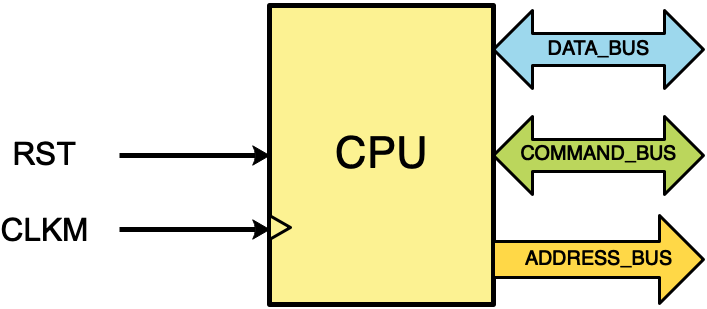
\includegraphics[scale=0.5]{1_prima_istanziazione}
	%\caption{Gesione della memoria in un'architettura di Von Neumann migliorata}
	\label{fig:prima_istanziazione}
\end{figure}
I segnali presenti a questo livello sono:
\begin{itemize}
	\item \textbf{OPERANDI E RISULTATO:}
	\begin{itemize}
		\item \textbf{DATA\_BUS} (N bit): bus dati di input-output connesso con il bus DATI di sistema.
		\item \textbf{COMMAND\_BUS} (N bit): bus contenente un raggruppamento dei segnali di controllo connesso con il bus COMANDI di sistema.
		\item \textbf{ADDRESS\_BUS} (2N bit): bus contenente i segnali di indirizzo per la memoria e le periferiche, connesso con il bus INDIRIZZI di sistema.
	\end{itemize}
	
	\item \textbf{CLOCK MACCHINA:}
	\begin{itemize}
		\item \textbf{CLKM}: clock macchina per evoluzione sincrona.
	\end{itemize}
	
	\item \textbf{RESET:}
	\begin{itemize}
		\item \textbf{RST}: \{0: funzionamento normale; 1: reset attivo $\rightarrow$ il sistema riavvia l'esecuzione dalla prima istruzione\}.
	\end{itemize}
\end{itemize}

\section{Regola protocollare}
\begin{itemize}
	\item \textit{ESTERNO}:
	\begin{enumerate}
		\item La macchina procede con l'esecuzione del programma salvato nella memoria RAM in modo sequenziale evolvendo con gli impulsi di clock esterni.
	\end{enumerate}

	\item \textit{INTERNO}:
	La CPU si trova nella condizione di reset e genera l'indirizzo 0000h per la memoria. Tale locazione conterrà la prima istruzione del programma scritto in RAM. Per ogni istruzione si esegue il ciclo di fetch-execute:
	\begin{enumerate}
		\item FETCH: La CPU preleva l'istruzione dalla memoria all'indirizzo fornito dal PC e la salva nel registro istruzione IR. Infine esegue un aggiornamento del PC.
		\item DECODE: La CPU riconosce l'istruzione e si occupa del prelievo eventuale dei dati dalla memoria salvandoli nei registri di appoggio interno.
		\item EXECUTE: La CPU esegue l'istruzione.
		\item (se previsto) WRITE-BACK: La CPU si occupa del salvataggio del dato sulla memoria.
	\end{enumerate}
\end{itemize}

\section {Task eseguibili, set di istruzioni e organizzazione della RAM interna}
In questa sezione ci si occupa di definire parte del set di istruzioni relativo a quanto discusso nel paragrafo \textquotedblleft Metodi di indirizzamento" di pagina \pageref{metodi_di_indirizzamento}. Riassumendo i task da eseguire e considerando i dati relativi a tali istruzioni si ottiene la seguente tabella.
\begin{table}[H]
	\centering
	\footnotesize
	\fontsize{10}{18}\selectfont
	\begin{tabular}{|p{0.5cm}|p{0.5cm}|p{0.5cm}|p{0.5cm}|p{0.5cm}|p{0.5cm}|}
		\hline
		\multicolumn{1}{|c|}{\textbf{INSTRUCTION}} & \multicolumn{1}{c|}{\textbf{CODE}} & 
		\multicolumn{3}{c|}{\textbf{BINARY EQUIVALENT}} & \multicolumn{1}{l|}{\textbf{MODIFIERS}} \\
		
		& & \multicolumn{1}{|c|}{COD. OP}  & \multicolumn{1}{|c|}{1st nibble} & \multicolumn{1}{|c|}{2nd nibble} & 	 \\ \hline
		
		\multicolumn{1}{|l|}{No operation}	&
		\multicolumn{1}{|c|}{NOP}  &
		\multicolumn{1}{|c|}{0000}	&
		\multicolumn{1}{|c|}{-} &
		\multicolumn{1}{|c|}{-} &
%		\multicolumn{1}{|c|}{-} &
		\multicolumn{1}{|c|}{-}	\\ \hline
		
		
		\multicolumn{1}{|l|}{Read RAM}	&
		\multicolumn{1}{|c|}{RD}  &
		\multicolumn{1}{|c|}{0001}	&
		\multicolumn{1}{|c|}{$A_7A_6A_5A_4$} &
		\multicolumn{1}{|c|}{$A_3A_2A_1A_0$} &
%		\multicolumn{1}{|c|}{-} &
		\multicolumn{1}{|l|}{address}	\\ \hline
		
		\multicolumn{1}{|l|}{Write RAM at address}	&
		\multicolumn{1}{|c|}{WR}  &
		\multicolumn{1}{|c|}{0011}	&
		\multicolumn{1}{|c|}{$A_7A_6A_5A_4$} &
		\multicolumn{1}{|c|}{$A_3A_2A_1A_0$} &
%		\multicolumn{1}{|c|}{$D_3D_2D_1D_0$} &	
		\multicolumn{1}{|l|}{address, data}	\\ \hline
		
		\multicolumn{1}{|l|}{Jump at Address}	&
		\multicolumn{1}{|c|}{JPA}  &
		\multicolumn{1}{|c|}{0100}	&
		\multicolumn{1}{|c|}{$A_7A_6A_5A_4$} &
		\multicolumn{1}{|c|}{$A_3A_2A_1A_0$} &
%		\multicolumn{1}{|c|}{-} &
		\multicolumn{1}{|l|}{address}	\\ \hline
		
		\multicolumn{1}{|l|}{Jump Offset}	&
		\multicolumn{1}{|c|}{JPO}  &
		\multicolumn{1}{|c|}{0101}	&
		\multicolumn{1}{|c|}{$O_3O_2O_1O_0$} &
		\multicolumn{1}{|c|}{-} &
%		\multicolumn{1}{|c|}{-} &
		\multicolumn{1}{|l|}{offset}	\\ \hline
		
		\multicolumn{1}{|l|}{Jump at Base+Offset}	&
		\multicolumn{1}{|c|}{JBO}  &
		\multicolumn{1}{|c|}{0111}	&
		\multicolumn{1}{|c|}{$O_3O_2O_1O_0$} &
		\multicolumn{1}{|c|}{$B_3B_2B_1B_0$} &
%		\multicolumn{1}{|c|}{-} &
		\multicolumn{1}{|l|}{offset, base}	\\ \hline
		
		\multicolumn{1}{|l|}{Move reg A to B}	&
		\multicolumn{1}{|c|}{MV}  &
		\multicolumn{1}{|c|}{1000}	&
		\multicolumn{1}{|c|}{$A_3A_2A_1A_0$} &
		\multicolumn{1}{|c|}{$B_3B_2B_1B_0$} &
%		\multicolumn{1}{|c|}{-} &
		\multicolumn{1}{|l|}{reg. A, reg. B}	\\ \hline
	\end{tabular}
	\caption{Set di istruzioni}
\end{table} 		
\noindent
Il numero di bit riservato al codice operazione è sovradimensionato rispetto al numero di operazioni. Per discriminare tra le operazioni possibili sarebbero stati sufficienti $\lceil log_2{7} \rceil = 3$ bit; tuttavia considerando la futura ed eventuale aggiunta di ulteriori istruzioni, nonchè il fatto di avere un bus dati a 4 bit, si è scelto di mantenere un codice operazione a 4 bit.\\
Come si può notare dalla tabella precedente sistema lavora su istruzioni operanti su 0, 1, o 2operandi a 4 bit. Sarà dunque compito della UC interna, una volta prelevata l'istruzione ed eseguita la decodifica, richiedere il numero di dati necessari all'esecuzione dell'istruzione stessa.
\par \bigskip \noindent
Si ricorda che la memoria è organizzata come in Figura \ref{fig:vn_mem}, dunque le istruzioni del programma troveranno posto in modo sequenziale nell'area \textquotedblleft istruzioni", così come i dati nell'area \textquotedblleft dati" sottostante. 
Poiché si dispone di un bus dati a 4 bit, nelle istruzioni dove si debba prelevare un indirizzo dalla memoria, si necessita di più accessi a locazioni di memoria contigue presenti all'area dati.
Si suppone dunque che la fase di traduzione da codice assembler a linguaggio macchina tenga conto di tale questione, procedendo ad inserire i dati nell'area di memoria dedicata ordinati in maniera sequenziale.

\section{Strategia e problematiche}
La struttura interna della CPU sarà ricavata in questo paragrafo tenendo conto del set di istruzioni e delle prerogative di progetto.\\
Anzitutto poiché dati e programmi sono reperiti a runtime dalla memoria RAM interna sarà necessario dotare la CPU di sistemi che permettano l'indirizzamento della memoria ai programmi ed al dato. In particolare si necessiterà quindi di due puntatori: un \textquotedblleft program counter" ed un \textquotedblleft data counter". Il PC conterrà l'indirizzo relativo alla prossima istruzione da eseguire, mentre il DC contiene l'indirizzo relativo al dato da prelevare.
In generale si può considerare che l'indirizzo per la lettura/scrittura della memoria può avere tre sorgenti:
\begin{itemize}
	\item il PC: come nel caso del prelievo delle istruzioni.
	\item il DC: come nel caso del prelievo/scrittura dei dati.
	\item un indirizzo generato internamente dalla CPU, ad esempio a seguito di un calcolo.
\end{itemize}
A tal proposito, nel procedere al corretto indirizzamento della memoria, l'uscita del bus indirizzi sarà pilotata da un registro al cui ingresso è presente un multiplexer controllato dalla UC interna col fine di discriminare quale dei tre registri sorgenti contenga il valore col quale indirizzare la memoria.\\
Entrambi i registri PC e DC, devono essere aggiornati (incrementati di 1) ad ogni prelievo relativamente di un'istruzione o di un dato. A tal proposito si doteranno entrambi i registri della possibilità di auto-incremento affiancando agli stessi un sommatore semplice.\\
Per dotare la CPU della possibilità di indirizzare la memoria da programma (come nel caso della RD e della WR) si può pensare di connettere uno dei registri interni presenti nel banco d'appoggio al mux di selezione. In tale caso l'indirizzamento della memoria sarà possibile senza compromettere i valori presenti in PC e DC. Tale registro avrà la funzione speciale di poter indirizzare la memoria e la sua etichetta sarà definita AR0.
\par \bigskip \noindent
Nel caso dell'operazione di RD l'indirizzo di lettura si suppone già presente nel registro AR0. Successivamente si effettua una lettura a tale indirizzo salvando il dato proveniente dalla RAM sul registro bidirezionale in/out.
Nel caso dell'operazione di WR si suppone che il dato da salvare sia già stato precaricato all'interno del registro bidirezionale in/out che pilota il bus dati dal lato CPU. Come nel caso della read, l'indirizzo su cui salvare il dato sarà stato precedentemente posto in AR0. L'operazione termina abilitando la memoria al salvataggio del dato su tale indirizzo.
\par \bigskip \noindent
Nel caso della jump immediata l'indirizzo di salto è indicato dal valore del dato prelevato dalla memoria. Il valore su cui effettuare il salto viene dapprima composto unendo le due letture della memoria che forniscono le due sottoparti dell'indirizzo nel registro AR0. Successivamente il PC verrà aggiornato al valore contenuto in AR0, indirizzato su di esso tramite multiplexer.
\par \bigskip \noindent
Nel caso delle operazioni denominate JPO e JBO il risultato del salto è dato dalla somma di un indirizzo \textquotedblleft \textit{base}" e di un \textit{offset} riferito a tale base. A seguito di una o due letture necessarie al caricamento di offset e base ed al caricamento di queste in due particolari registri di appoggio denominati DRO e DRB il valore di PC viene aggiornato a quello corretto eseguendo il calcolo del nuovo indirizzo su di una unità di calcolo ausiliare. In questo modo non si necessiterà dell'impiego della ALU principale nel caso di calcolo di tali indirizzi di salto. Il collegamento elettrico che permette l'incremento del PC al valore corretto è presentato nel successivo schema di seconda istanziazione.
\par \bigskip \noindent
Infine, considerando la struttura elementare interna di un'architettura di Von Neumann come quella riportata in Figura \ref{fig:vn_cpu}, la CPU contiene al suo interno un banco di registri di appoggio al calcolo. In particolare, nel caso relativo a questo esercizio, oltre ai già noti PC e DC trovano posto:
\begin{itemize}
	\item 10 registri di appoggio per i dati con etichetta.
	\item 1 registro accumulatore ACC.
	\item 4 registri di supporto al calcolo di ADDR, tra cui AR0.
	\item 1 registro bidirezionale per il salvataggio dei dati in ingresso/uscita, connesso al bus dati di sistema.
\end{itemize}
Su tutti questi registri si applica l'operazione di move parametrica (COD. OP: MV), la quale eseguirà la copia del contenuto di uno dei registri sorgente in un altro di destinazione, ad eccezione del registro ACC che fungerà solo da destinazione e non da sorgente. Per l'esecuzione di tale operazione si può pensare di inserire all'interno dell'area dedicata ai registri una logica combinatoria che apra il \textquotedblleft canale di transito" al dato dal registro sorgente a quello destinazione. Uno strobe da parte della UC master sul registro destinazione ne copierà il dato all'interno completando l'operazione. Per discriminare i registri coinvolgibili in tale operazione si doterà ognuno di questi di una etichetta caratteristica, ossia definita a livello di microcodice. Al programmatore sarà sufficiente scrivere i tag dei registi opportuni nella programmazione a livello assembler per garantire la riuscita dell'operazione in modo corretto.
\par \bigskip \noindent
Detto questo si può procedere alla seconda istanziazione della CPU.
\chapter{Seconda istanziazione}
\section{Schema a blocchi e definizione dei segnali IN/OUT}
A partire da quanto esposto nel precedente capitolo segue lo schema di seconda istanziazione della CPU.
%\newpage
\subsection{Schema a blocchi}
\begin{figure}[H]
	\centering
	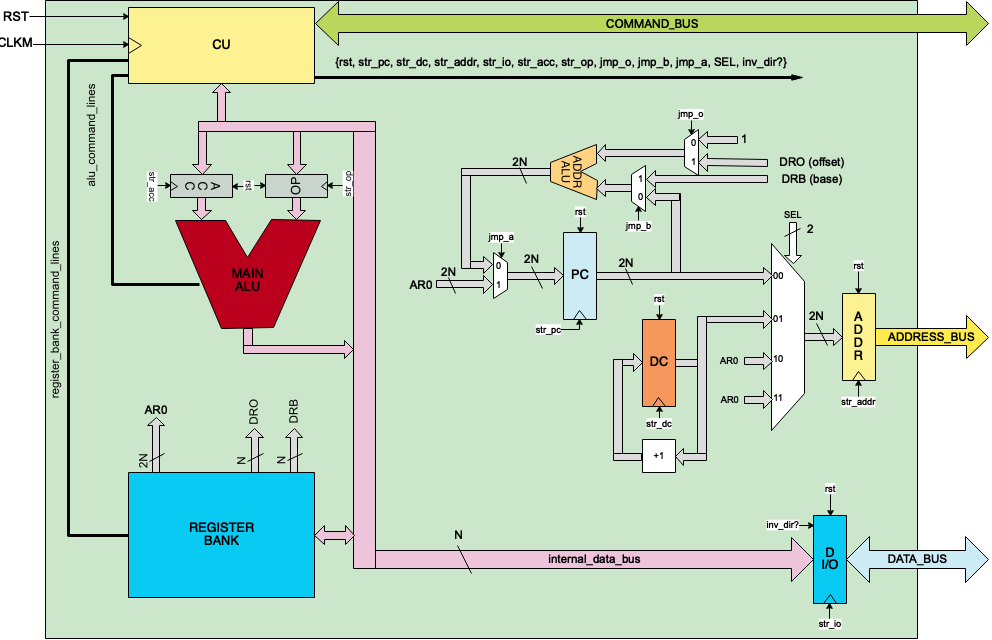
\includegraphics[scale=0.56, angle=90]{2_seconda_istanziazione}
	\label{fig:seconda_istanziazione}
\end{figure}

\newpage
\subsection{Segnali interni}
I segnali interni presenti a questo livello sono i seguenti.
\begin{itemize}
	\item \textit{rst}: \{0: funzionamento normale; 1: reset prioritario per i registri interni\}.
	\item \textit{str\_pc}: strobe per il registro PC.
	\item \textit{str\_dc}: strobe per il registro DC.
	\item \textit{str\_addr}: strobe per il registro address.
	\item \textit{str\_io}: strobe per il registro di I/O.
	\item \textit{str\_acc}: strobe per il registro accumulatore.
	\item \textit{str\_op}: strobe per il registro operando.
	\item \textit{jmp\_o}: segnale di comando per il mux. \{0: uscita = 1, 1: uscita = \textit{DRO}\}.
	\item \textit{jmp\_b}: segnale di comando per il mux. \{0: uscita = PC, 1: uscita = \textit{DRB}\}.
	\item \textit{jmp\_a}: segnale di comando per il mux. \{0: uscita = \textit{ALU\_ADDR\_OUT}, 1: uscita = \textit{AR0}\}.
	\item \textit{\textbf{SEL}}: 2 bit. Segnale di comando per il mux selezione indirizzo. Vedi \ref{2_tabella_SEL}.
	\item \textit{inv\_dir?}: \{0: registro I/O in funzionamento IN $\rightarrow$ OUT; 1: registro I/O in funzionamento OUT $\rightarrow$ IN\}.
	\item \textit{\textbf{alu\_command\_lines}}: linee di controllo per la ALU principale.
	\item \textit{\textbf{register\_bank\_command\_lines}}: linee di controllo per il register bank.
	\item \textit{\textbf{internal\_data\_lines}}: Bus dati interno a N bit.
\end{itemize}

\section{Ulteriori considerazioni di seconda istanziazione}
Per ciò che concerne l'indirizzamento della memoria si può notare che il registro indirizzo è pilotato da un mux 4-1, controllato tramite \textit{\textbf{SEL}}. \textit{\textbf{SEL}} è un segnale a 2 bit proveniente dalla CU ed il controllo del mux è schematizzato nella seguente tabella:
\begin{table}[H]
	\centering
	\footnotesize
	\fontsize{10}{18}\selectfont
	\begin{tabular}{|p{1.5cm}|p{1.5cm}|p{2.5cm}|}
		\hline
		\multicolumn{1}{|c|}{\textit{$SEL_1$}} &
		\multicolumn{1}{c|}{\textit{$SEL_0$}} & 
		\multicolumn{1}{c|}{SORGENTE ADDR}\\
		
		\hline
		\multicolumn{1}{|c|}{0} &
		\multicolumn{1}{c|}{0} & 
		\multicolumn{1}{c|}{\textbf{PC}}\\
		
		\hline
		\multicolumn{1}{|c|}{0} &
		\multicolumn{1}{c|}{1} & 
		\multicolumn{1}{c|}{\textbf{DC}}\\
		
		\hline
		\multicolumn{1}{|c|}{1} &
		\multicolumn{1}{c|}{0} & 
		\multicolumn{1}{c|}{\textbf{AR0}}\\
		
		\hline
		\multicolumn{1}{|c|}{1} &
		\multicolumn{1}{c|}{1} & 
		\multicolumn{1}{c|}{\textbf{AR0}}\\ \hline
	\end{tabular}
	\caption{Indirizzamento della memoria}
	\label{2_tabella_SEL}
\end{table}
\noindent
Questo perché, come detto, è necessario avere tre possibili sorgenti per l'indirizzamento della memoria. Il valore di indirizzamento proviene da PC, DC oppure da AR0, nei casi in cui $SEL_1$ = 1. AR0 è uno dei tre registri presenti nel banco d'appoggio con \textquotedblleft funzione speciale", ossia connesso ad un bus esterno accessibile in modo prioritario, proprio per avere la possibilità di realizzare funzioni come l'indirizzamento della memoria o il caricamento del valore del salto nel caso della jump.

\section{Dimensionamento interno dei blocchi di seconda istanziazione}
\subsection{Register bank}
\begin{figure}[H]
	\centering
	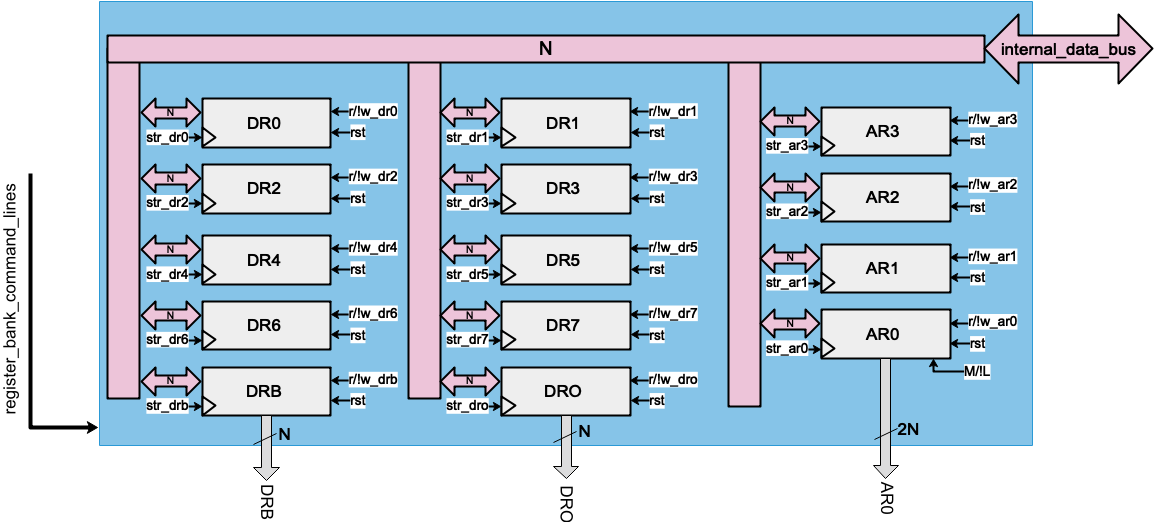
\includegraphics[scale=0.35, angle=0]{2_register_bank}
	\label{fig:register_bank}
\end{figure}
Il register bank contiene 14 registri di supporto al calcolo, di cui 4 riservati al calcolo degli indirizzi. Tra di essi vi sono tre registri accessibili esternamente attraverso altrettanti bus dedicati. Tali registri sono:
\begin{itemize}
	\item DRB: nel caso dell'operazione JBO in questo registro è presente il valore relativo alla base da sommare all'offset per il calcolo dell'indirizzo di salto.
	\item DRO: nel caso delle operazioni di JPO o JBO in questo registro è presente il valore relativo all'offset da sommare al PC o alla base per il calcolo dell'indirizzo di salto.
	\item AR0: in questo registo è presente il valore da dare al PC nel caso di jump immediata, oppure il valore da fornire alla memoria nel caso di RD o WR. Questo registro ha dimensione 2N bit per garantire l'indirizzamento a tutta la memoria, tuttavia è collegato attraverso il bus dati interno solo agli ultimi N bit. Attraverso il comando denominato $M/\overline{L}$ indirizzare il bus dati in scrittura ai primi N flip-flop o agli ultimi N flip-flop che compongono tale registro, per garantire il caricamento su tutto lo spazio dei 2N bit tramite bus a N bit. Di seguito sarà presentato lo schema interno-
\end{itemize}
Ogni registro componente il register bank è pilotato singolarmente attraverso una terna di segnali: \{\textit{str\_xxx}, \textit{rst}, \textit{r/$\overline{w}$\_xxx}\}. Nel caso del registro AR0 è presente anche il segnale $M/\overline{L}$ il cui impiego è necessario per avere la possibilità di scrivere o leggere separatemente i LSH (Least Significant Heap) o gli MSH (Most Significant Heap), ossia gli ultimi/primi N bit del registro. Dettagli del funzionamento del registro AR0 saranno esposti in seguito.\\
L'insieme dei segnali di controllo è stato schematizzato nella figura con l'insieme di linee denominato \textit{\textbf{register\_bank\_command\_lines}}.\\
Ogni registro che compone il register bank è inoltre di tipo bidirezionale a singolo bus, per avere la possibilità di essere letto o scritto attraverso il bus dati interno. Lo schema interno del generico registro, supposto N=4 bit, è rappresentato nella figura seguente.
\begin{figure}[H]
	\centering
	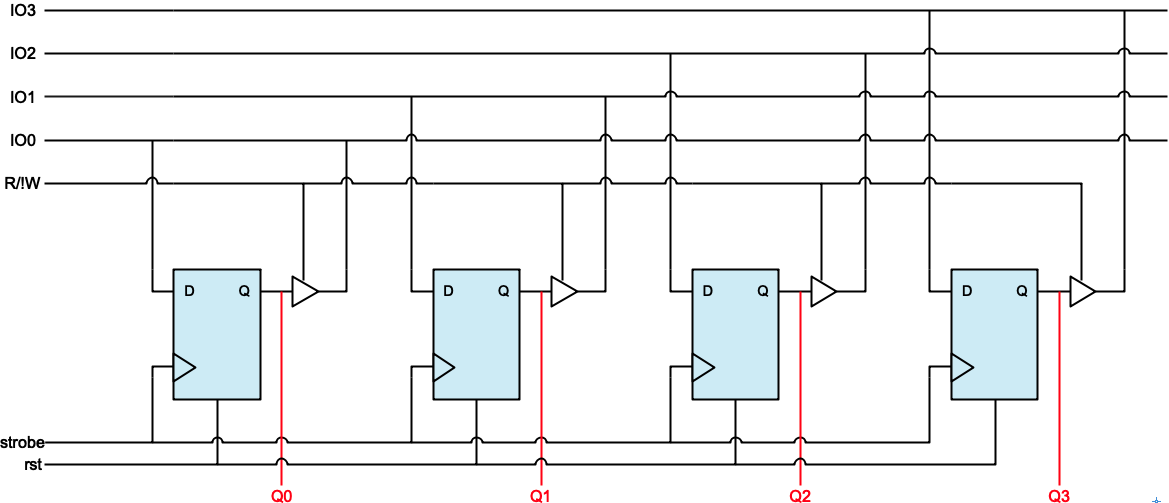
\includegraphics[scale=0.32, angle=0]{2_registro_bidir}
	\label{fig:registro_bidir}
\end{figure}
\noindent
In questo schema il comando $R/ \overline{W}$ definisce se il registro è abilitato alla lettura (1) o alla scrittura (0), in modo che il bus possa essere bidirezionale. Quando un registro non è utilizzato deve essere mantenuto in modalità scrittura ($R/ \overline{W} = 0$) per far si che i tri-state d'uscita siano disabilitati in modo da non interferire col controllo del bus da parte di altre entità ad esso collegate.
\\
In rosso invece sono rappresentate le linee d'uscita disponibili solamente per i registri con accesso speciale DRO e DRB, che costituiscono i bus dedicati discussi in precedenza.\\
Lo schema interno del registro AR0 (rappresentato per N=2 bit) è invece il seguente. Si ricorda che la dimensione di tale registro è pari a 2N bit, dunque:
\begin{figure}[H]
	\centering
	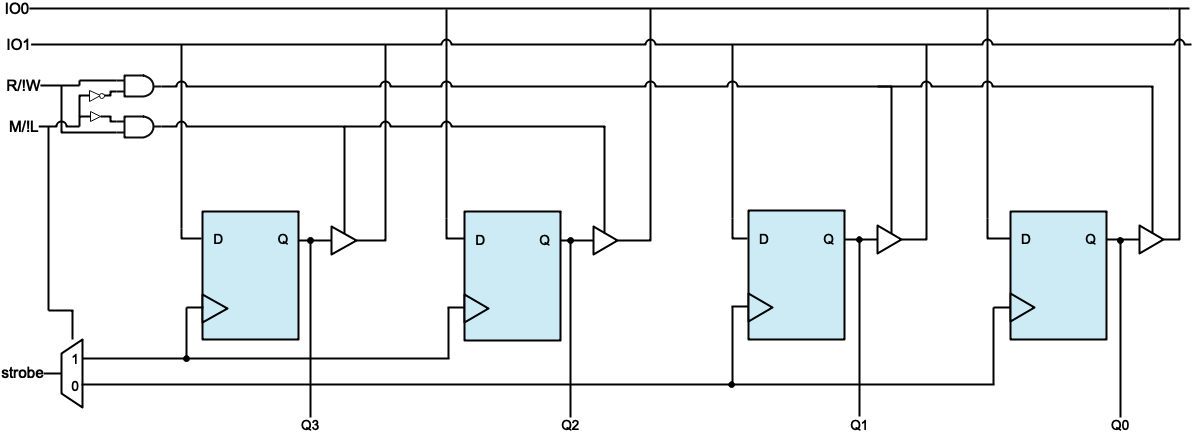
\includegraphics[scale=0.32, angle=0]{2_AR0}
	\label{fig:AR0}
\end{figure}
\noindent
Si può notare il demultiplexer interno che permette lo smistamento del segnale di strobe indipendentemente al primo o al secondo gruppo di flip-flop e la rete logica che pilota i tri-state che realizza la seguente funzione.
\begin{table}[H]
	\centering
	\fontsize{10}{18}\selectfont
	\begin{tabular}{|p{5mm}|p{5mm}|p{25mm}|}
		\hline
		\multicolumn{1}{|c|}{\textit{$R/\overline{W}$}} &
		\multicolumn{1}{c|}{\textit{$M/\overline{L}$}} & 
		\multicolumn{1}{c|}{\textbf{modalità}}\\
		
		\hline
		\multicolumn{1}{|c|}{0} &
		\multicolumn{1}{|c|}{0} & 
		\multicolumn{1}{c|}{scrittura LSH}\\
		
		\hline
		\multicolumn{1}{|c|}{0} &
		\multicolumn{1}{|c|}{1} & 
		\multicolumn{1}{c|}{scrittura MSH}\\
		
		\hline
		\multicolumn{1}{|c|}{1} &
		\multicolumn{1}{|c|}{0} & 
		\multicolumn{1}{c|}{lettura LSH}\\
		
		\hline
		\multicolumn{1}{|c|}{1} &
		\multicolumn{1}{|c|}{1} & 
		\multicolumn{1}{c|}{lettura MSH}\\ \hline
	\end{tabular}
	\caption{Modalità di funzionamento registro AR0}
\end{table}
\noindent
Omesso dal disegno, ma presente, il clear prioritario dei flip-flop connesso al segnale esterno di \textit{reset}.
\subsection{Registro IN-OUT}
Un'importante funzione è delegata al registro bidirezionale D$\_$I/O, ossia quella di pilotare il bus dati in uscita e fungere da pozzo per i dati in ingresso. Il registro deve dunque essere di tipo bidirezionale. Lo schema interno è il seguente.
\begin{figure}[H]
	\centering
	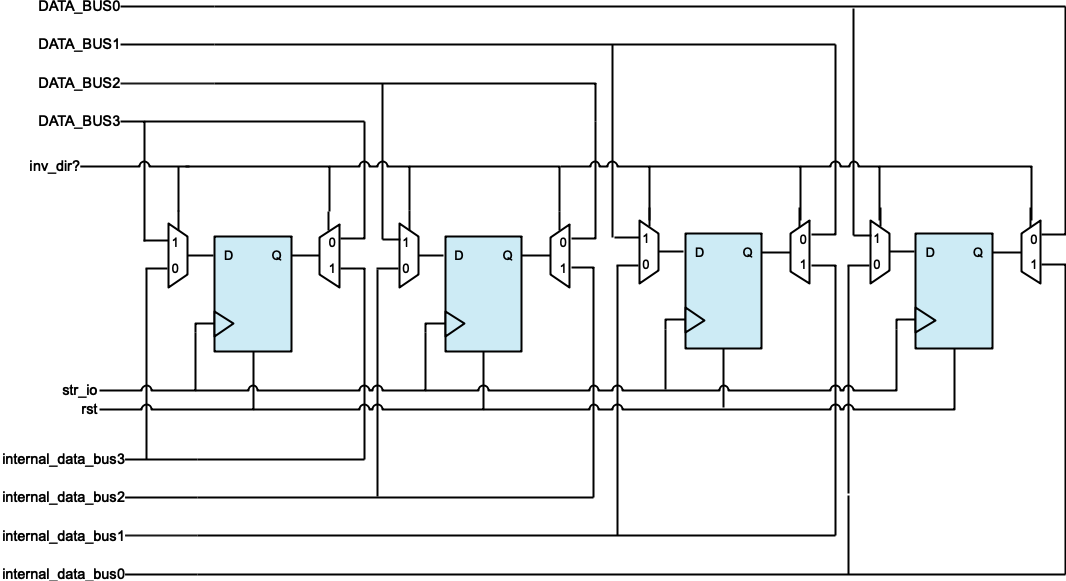
\includegraphics[scale=0.35, angle=0]{2_dio}
	\label{fig:dio}
\end{figure}
\noindent
Il registro non è dotato di buffer tri-state in ingresso/uscita, dunque sarà necessario fare in modo che questo sia sempre in modalità \textit{inv$\_$dir? = 0} quando non è in utilizzo.

\subsection{Unità di controllo: CU}
\begin{figure}[H]
	\centering
	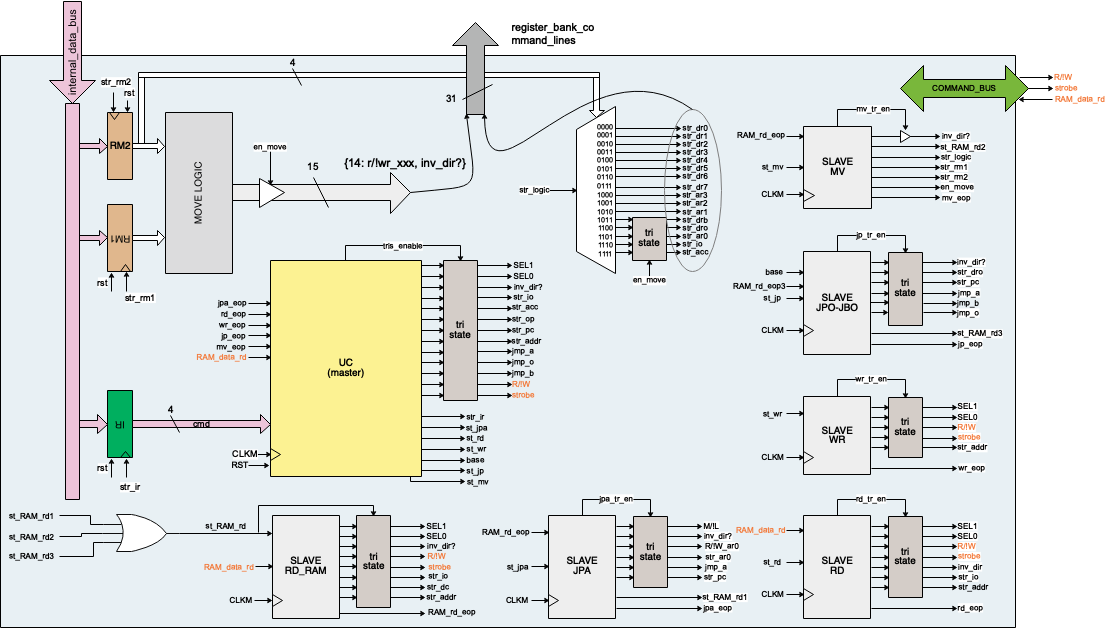
\includegraphics[scale=0.47, angle=90]{2_cu}
	\label{fig:cu}
\end{figure}
\newpage
\subsubsection{Segnali interni}
I segnali interni che trovano posto all'interno dello schema di terza istanziazione della UC sono i seguenti:
\begin{itemize}
	\item \textit{rst}: \{0: funzionamento normale; 1: reset prioritario per tutti i registri\}.
	\item \textit{str$\_$ir}: strobe per il registro istruzioni IR.
	\item \textit{\textbf{cmd}}: uscita a 4 bit dell'IR.
	\item \textit{str$\_$rm1}: strobe per il registro di supporto alla move RM1.
	\item \textit{str$\_$rm2}: strobe per il registro di supporto alla move RM2.
	\item \textit{st$\_$nomeslave}: segnale di start per lo slave \textit{nomeslave}. Delega il comando da parte della UC master allo slave \textit{nomeslave} per l'esecuzione del proprio task.
	\item \textit{nomeslave$\_$eop}: se 1 indica che lo slave \textit{nomeslave} ha terminato l'esecuzione delle proprie operazioni.
	\item \textit{base}: \{1: indica allo slave JPO/JBO se è richiesta una somma con base (JBO) prelevata dalla memoria; 0: somma JPO semplice\}\item \textit{nomeslave$\_$tr$\_$en}: lo slave \textit{nomeslave} abilita il proprio banco di buffer tri-state per pilotare le linee condivise.
	\item \textit{en$\_$move}: abilitazione dei tri-state per la logica di move.
	\item \textit{str$\_$logic}: strobe per il demux di move, esegue la copia del dato sul registro destinazione.
	\item \textit{str$\_$nomeregistro}: strobe per il registro \textit{nomeregistro}, appartenente al register bank.
	\item \textit{st$\_$RAM$\_$rdX}: segnale per lo start dello slave RD$\_$RAM. Vi sono 3 segnali provenienti da altrettanti slave che all'occorrenza abilitano RD$\_$RAM. L'abilitazione avviene tramite operazione di OR su questi tre segnali.
\end{itemize}
Inoltre, connessi al BUS COMANDI si trovano i segnali di controllo per la RAM:
\begin{itemize}
	\item \textit{R/$\overline{W}$}: \{0: abilitata scrittura della memoria RAM interna alla CPU; 1: RAM abilitata alla lettura.\}.
	\item \textit{strobe}: strobe per la memoria RAM.
	\item \textit{RAM$\_$data$\_$rd}: \{1: la RAM ha terminato la lettura o e il dato è disponibile sul BUS DATI di sistema; 0: la RAM è in stato \textit{busy}\}.
\end{itemize}

Passiamo ora a definire i diagrammi ASM per le MSF slave interne alla UC.
\subsubsection{Slave RD$\_$RAM}
Esegue la lettura della memoria di un dato indirizzando la RAM tramite il DC. Il diagramma ASM è il seguente.
\begin{figure}[H]
	\centering
	\includegraphics[scale=0.5]{ASM_ram_rd}
	\label{fig:asm_ram_rd}
\end{figure}

\newpage
\subsubsection{Slave JPA}
Esegue la jump immediata, aggiornando il Program Counter all'indirizzo di salto ricavato dalla memoria.
\begin{figure}[H]
	\centering
	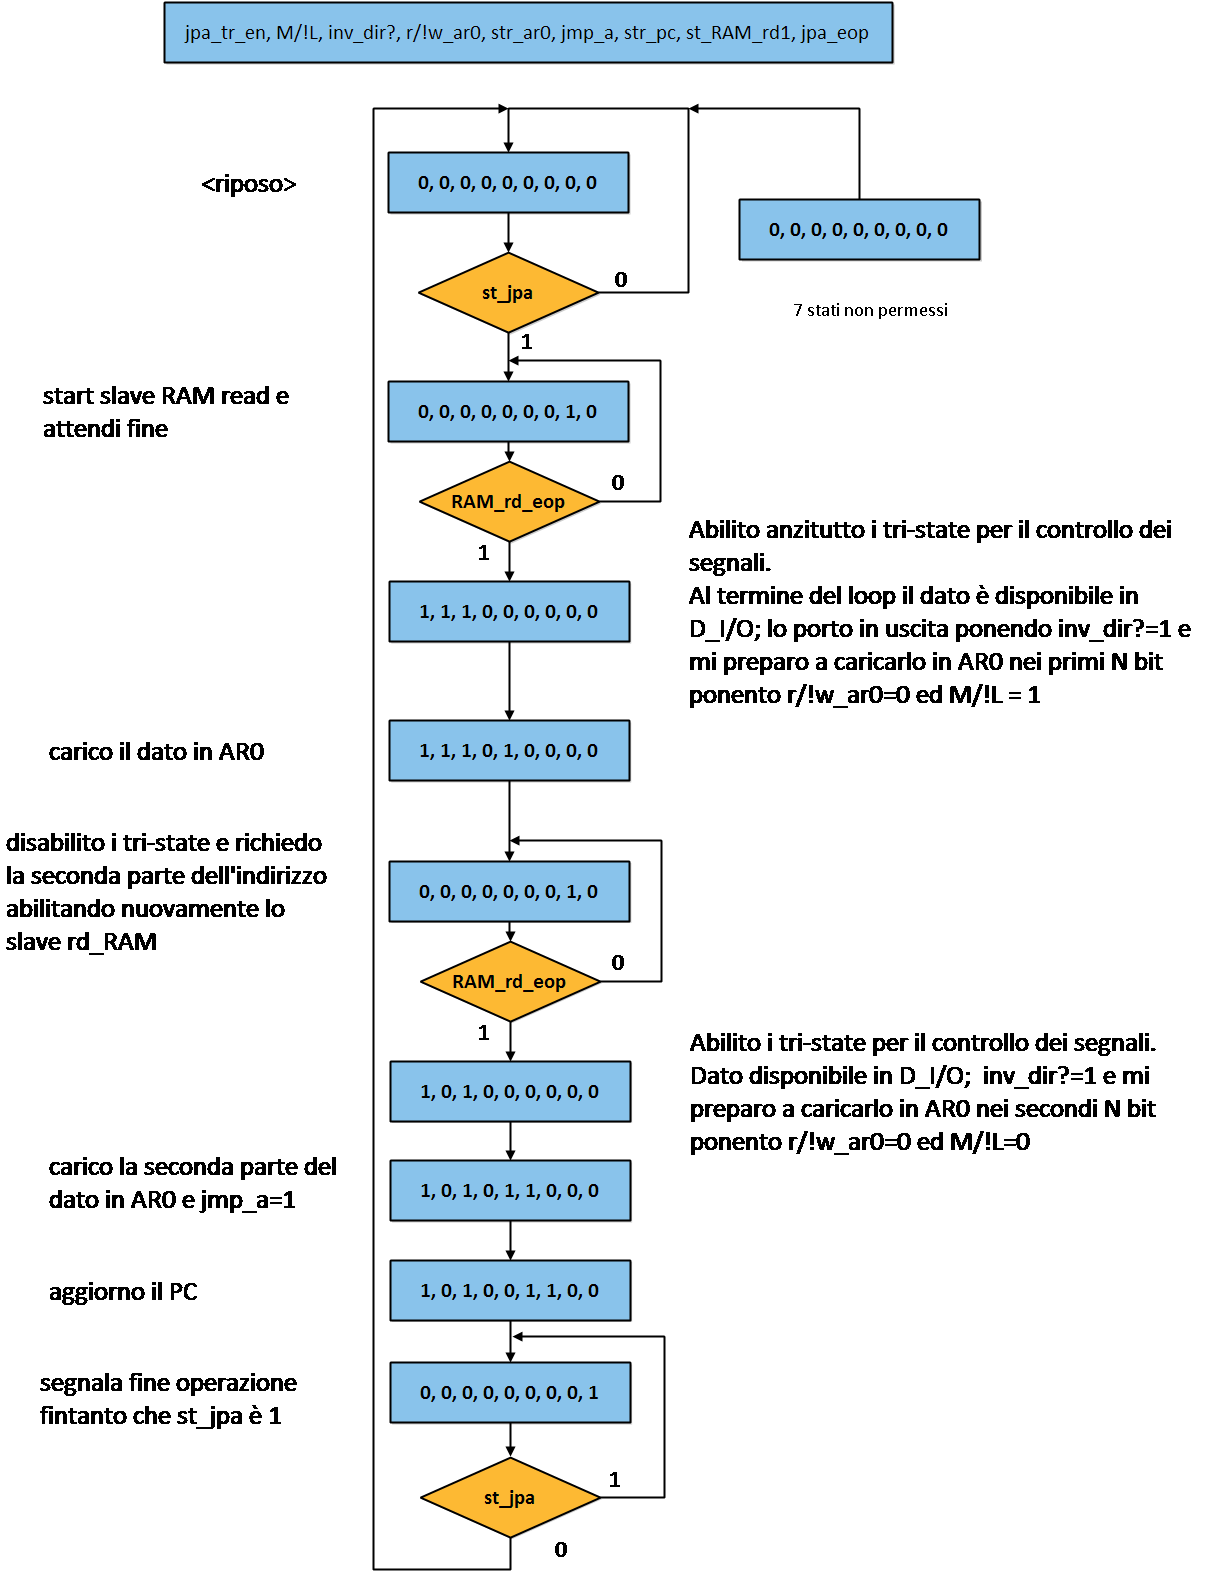
\includegraphics[scale=0.43]{asm_jpa}
	\label{fig:asm_jpa}
\end{figure}

\newpage
\subsubsection{Slave RD}
Esegue la lettura della memoria all'indirizzo presente in AR0 e salva il dato sul registro D$\_$I/O.
\begin{figure}[H]
	\centering
	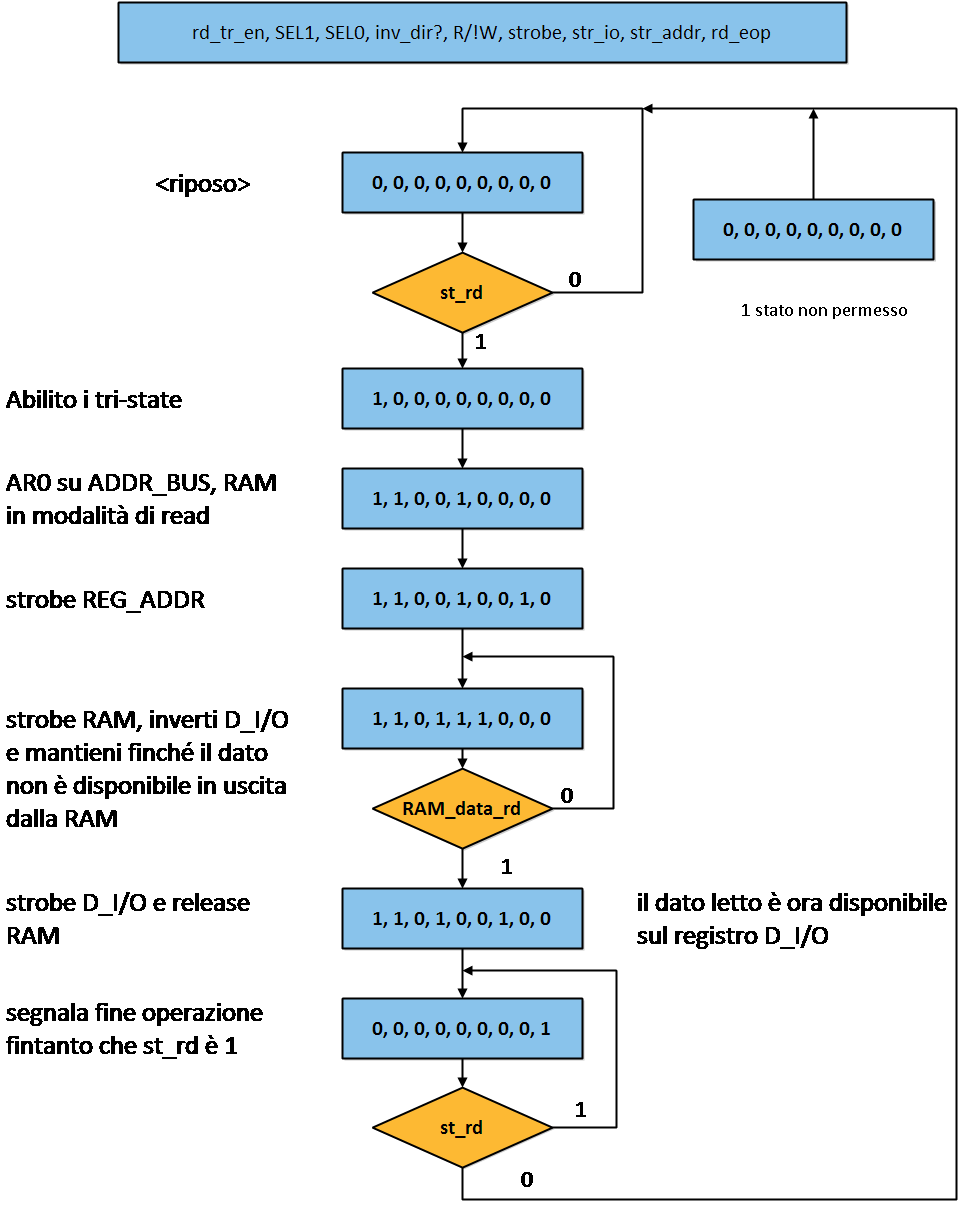
\includegraphics[scale=0.55]{asm_rd}
	\label{fig:asm_rd}
\end{figure}

\newpage
\subsubsection{Slave WR}
Esegue la scrittura del dato presente in D$\_$I/O nella memoria alla locazione imposta dall'indirizzo presente in AR0.
\begin{figure}[H]
\centering
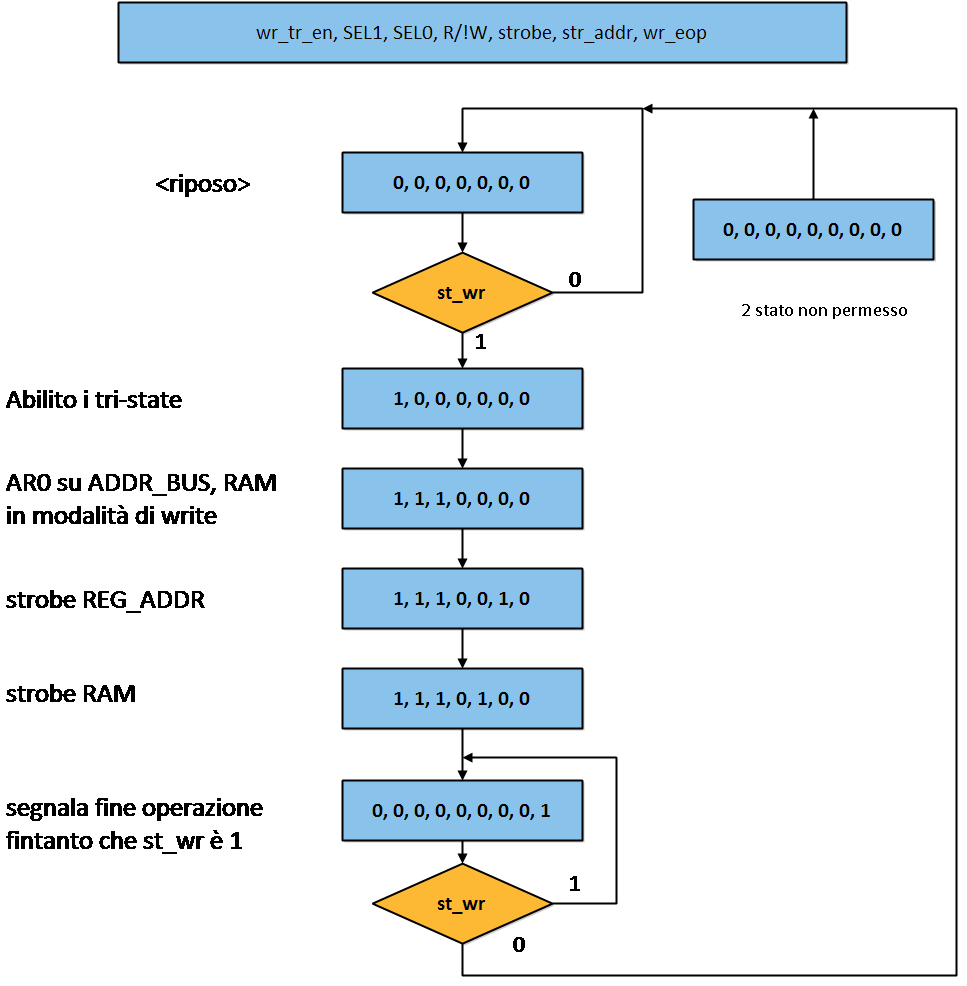
\includegraphics[scale=0.55]{asm_wr}
\label{fig:asm_wr}
\end{figure}

\newpage
\subsubsection{Slave JPO$\_$JBO}
Esegue la jump all'indirizzo dato dalla somma di una \textit{base} e un offset. Mentre l'offset proviene dalla memoria, la base può essere l'indirizzo corrente del PC o un ulteriore dato prelevato dalla memoria.
\begin{figure}[H]
	\centering
	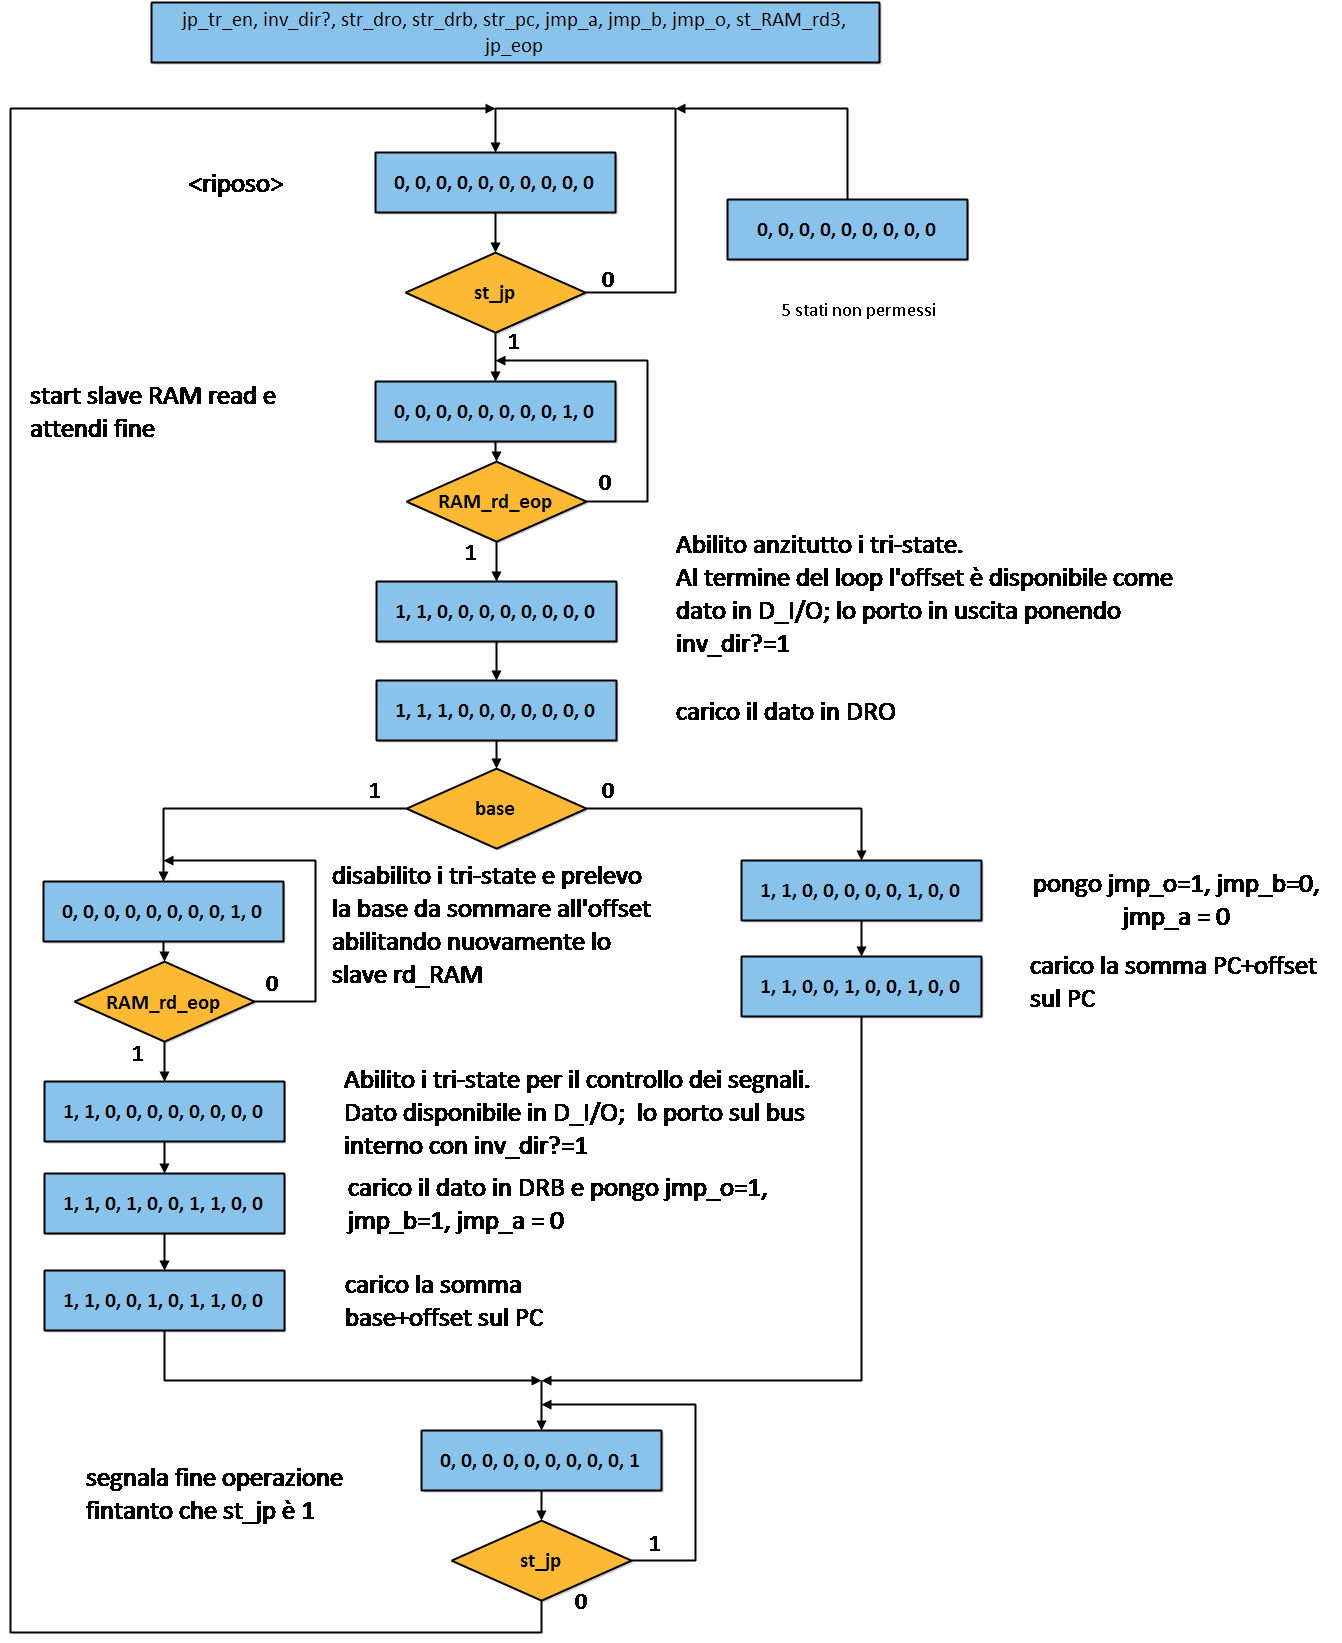
\includegraphics[scale=0.40]{asm_jp}
	\label{fig:asm_jp}
\end{figure}

\newpage
\subsubsection{Slave MV}
Esegue la copia del dato da un registro sorgente ad uno destinazione indirizzati tramite etichetta prelevata dalla memoria.
\begin{figure}[H]
	\centering
	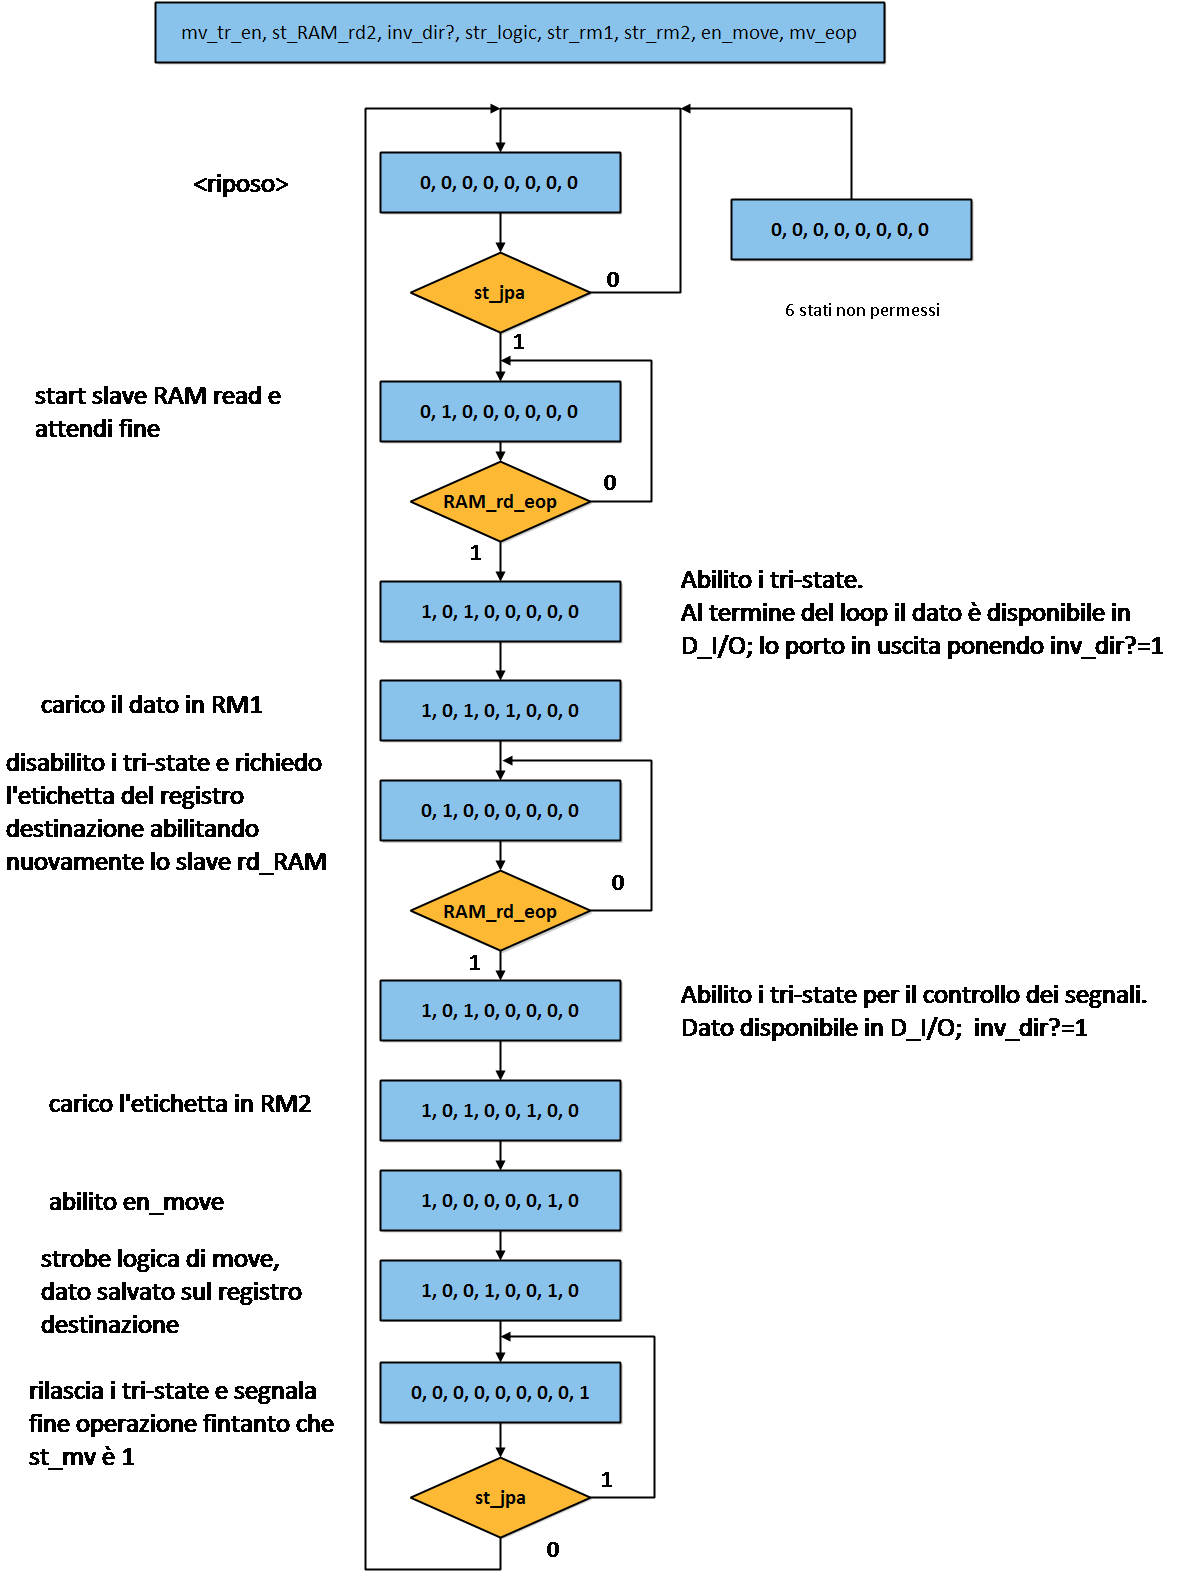
\includegraphics[scale=0.43]{asm_mv}
	\label{fig:asm_mv}
\end{figure}

\newpage
\subsubsection{ASM MASTER}
Infine, il diagramma ASM per la macchina master che esegue le fasi di fetch e decode, delegando l'execute agli slave. Le azioni da svolgere sono:\\
\par \bigskip \noindent
FETCH:
\begin{enumerate}
	\item Poni PC su ADDR$\_$BUS, RAM in modalità di read.
	\item Strobe REG$\_$ADDR
	\item RIPETI: Strobe RAM e poni inv$\_$dir=1 FINCHÉ RAM$\_$data$\_$rd = 1
	\item Strobe IR e incrementa PC
\end{enumerate}

\par \bigskip \noindent
DECODE:
\begin{enumerate}
	\item L'uscita del registro istruzioni IR contiene il codice relativo all'istruzione da eseguire. Una serie di controlli interni identifica l'operazione definita dai segnali di \textbf{\textit{cmd}}.
\end{enumerate}

\par \bigskip \noindent
EXECUTE (WRITE-BACK):
\begin{enumerate}
	\item Riconosciuta l'istruzione la macchina MASTER delega il controllo dell'hardware interno allo slave che eseguirà l'istruzione e cederà nuovamente il controllo alla master. Lo slave si occupa anche di un eventuale WRITE-BACK in memoria.
\end{enumerate}

\noindent
Da cui il diagramma ASM per la macchina MASTER.
\begin{figure}[H]
	\centering
	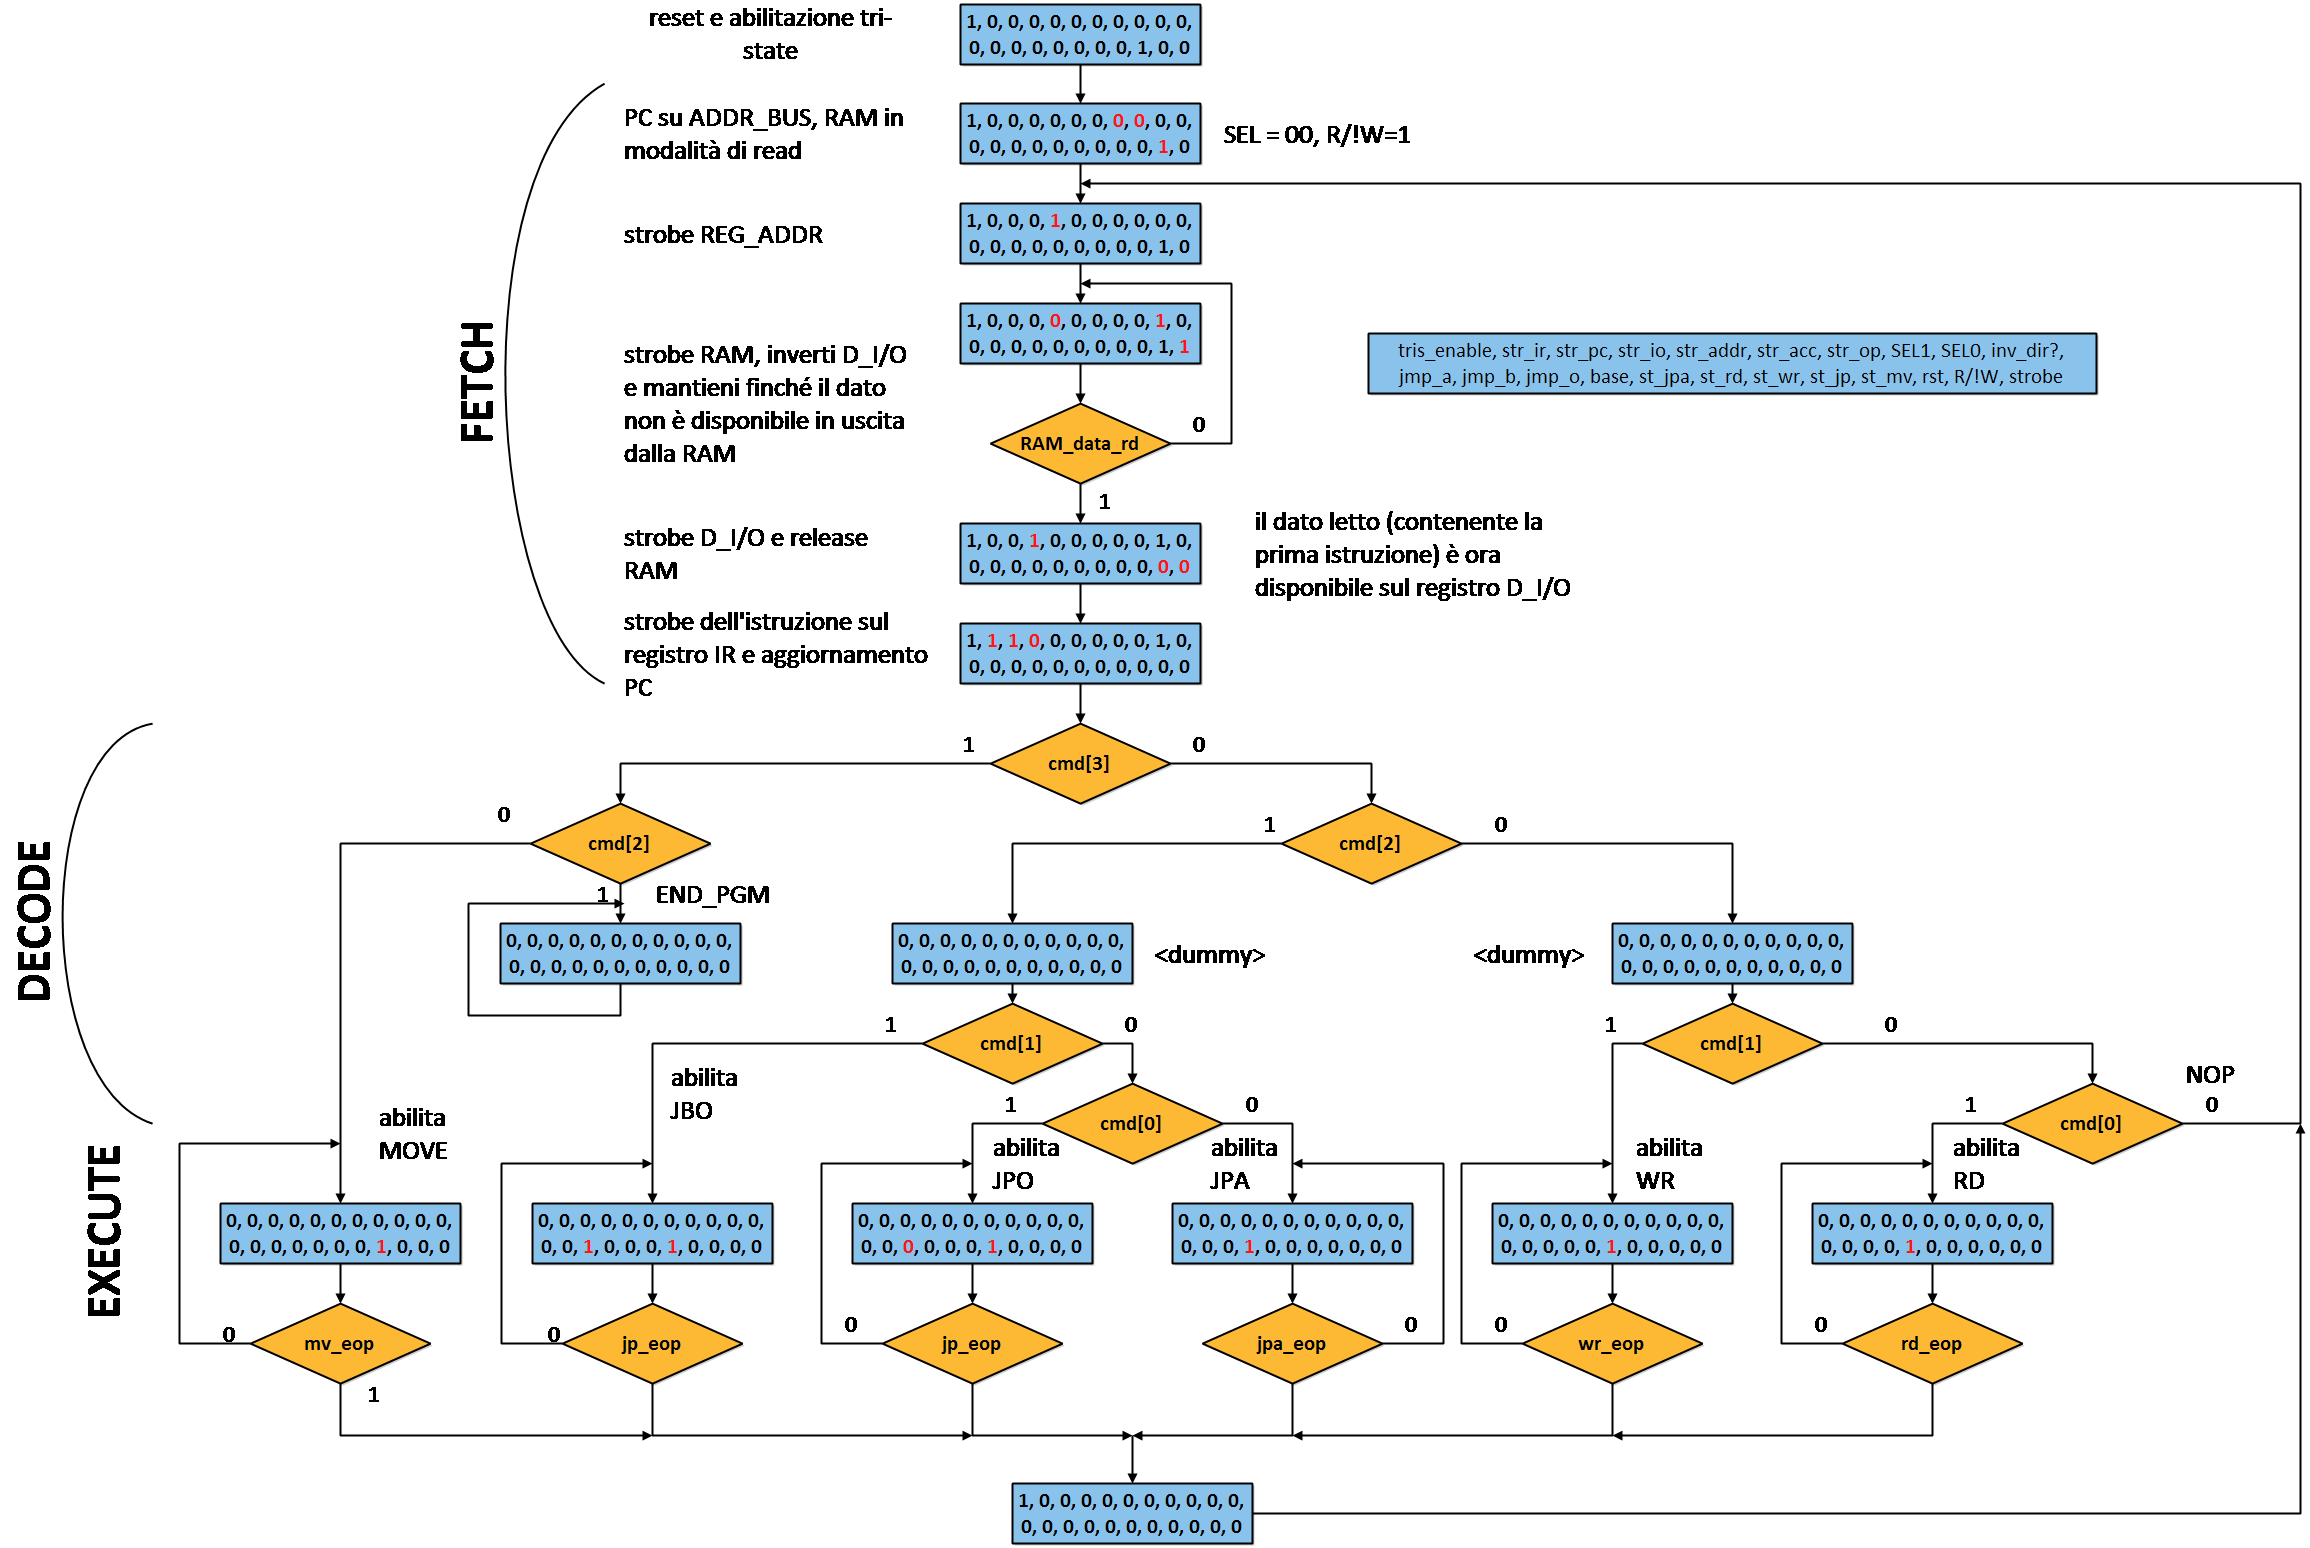
\includegraphics[scale=0.30, angle=90]{asm_master}
	\label{fig:asm_master}
\end{figure}



\end{document}  

%\input{Capitolo2}
%\input{Capitolo3}
%\input{Capitolo4}
%\input{Capitolo5}

%\newpage
%\listoffigures
%\addcontentsline{toc}{chapter}{Elenco delle figure}
%\listoftables
%\addcontentsline{toc}{chapter}{Elenco delle tabelle}
%\newpage

%\input{Ringraziamenti}
%\addcontentsline{toc}{chapter}{Ringraziamenti}

